%% 
%% Copyright 2007-2024 Elsevier Ltd
%% 
\newif\ifsnclass
\IfFileExists{sn-jnl.cls}{%
  \snclasstrue
	\documentclass[pdflatex,sn-mathphys,Numbered]{sn-jnl}
}{%
  \snclassfalse
  \documentclass[11pt]{article}
}
\usepackage{graphicx}
\usepackage{amsthm}
\usepackage{amsmath}
\usepackage{amsfonts}
\usepackage{amssymb}
\usepackage{xcolor}
\usepackage{textcomp}
\usepackage{manyfoot}
\usepackage{booktabs}
\usepackage{multirow}
\usepackage{tabularx}
\usepackage{chngcntr}
\usepackage[ruled,vlined]{algorithm2e}
\ifsnclass\else
\usepackage[numbers]{natbib}
\usepackage[papersize={210mm,297mm},margin=20mm]{geometry}
\fi
\setkeys{Gin}{draft=false}
\setlength{\emergencystretch}{2em}

\numberwithin{equation}{section}
\counterwithin{figure}{section}
\counterwithin{table}{section}
\newtheorem{theorem}{Theorem}
\ifsnclass\raggedbottom\else\renewcommand{\baselinestretch}{1.2}\fi
%\newtheorem{proof}{Proof}

%\journal{Nuclear Physics B}

\newcommand{\supphead}[1]{\ifsnclass\bmhead{#1}\else\section*{#1}\fi}
\newcommand{\enterbackmatter}{\ifsnclass\backmatter\fi}

\begin{document}
\ifsnclass
\title[Distributionally Robust MPC for Autonomous Driving]{Distributionally Robust Model Predictive Control with Disturbance Uncertainty Adaptiveness for Obstacle Avoidance of Autonomous Driving}

\author[1]{\fnm{Nan} \sur{Xue}}
\author*[2]{\fnm{Lei} \sur{Zhang}}\email{reizhg@tongji.edu.cn}
\affil[1]{\orgname{BA TechWorks, BMW Group}, \orgaddress{\city{Nanjing}, \country{China}}}
\affil*[2]{\orgdiv{State Key Laboratory of High-speed Maglev Transportation Technology}, \orgname{College of Electronic and Information Engineering, Tongji University}, \orgaddress{\city{Shanghai}, \country{China}}}

\abstract{This paper proposes a Koopman-based distributionally robust MPC framework for autonomous vehicle obstacle avoidance under disturbance uncertainty. The tracking objective is an empirical expected cost over historical disturbance trajectories. For each obstacle-time constraint, a shifted-hinge loss and Markov's inequality yield a conservative sufficient condition for a distributionally robust chance constraint over a first-order Wasserstein ambiguity set. For fixed safety-margin parameters, this condition results in affine safety constraints and preserves the convex QP structure. The simulation results in the current draft were generated with the previous safety formulation and will be replaced after rerunning the experiments under the revised condition.}

\keywords{Vehicle Dynamics, Distributionally Robust Model Predictive Control, Koopman Operator, Uncertainty Adaptiveness}

\maketitle
\else
\title{Distributionally Robust Model Predictive Control with Disturbance Uncertainty Adaptiveness for Obstacle Avoidance of Autonomous Driving}
\author{Nan Xue \and Lei Zhang\thanks{Corresponding author. IEEE Senior Member. ORCID: 0000-0003-1961-3176. Email: reizhg@tongji.edu.cn}}
\date{}
\maketitle

\begin{center}
\textit{State Key Laboratory of High-speed Maglev Transportation Technology, College of Electronic and Information Engineering, Tongji University, Shanghai, China}\\
\textit{BATechWorks, BMW Group, Nanjing, China}
\end{center}

\begin{abstract}
This paper proposes a Koopman-based distributionally robust MPC framework for autonomous vehicle obstacle avoidance under disturbance uncertainty. The tracking objective is an empirical expected cost over historical disturbance trajectories. For each obstacle-time constraint, a shifted-hinge loss and Markov's inequality yield a conservative sufficient condition for a distributionally robust chance constraint over a first-order Wasserstein ambiguity set. For fixed safety-margin parameters, this condition results in affine safety constraints and preserves the convex QP structure. The simulation results in the current draft were generated with the previous safety formulation and will be replaced after rerunning the experiments under the revised condition.
\end{abstract}

\noindent\textbf{Keywords:} Vehicle Dynamics; Distributionally Robust Model Predictive Control; Koopman Operator; Uncertainty Adaptiveness.

\bigskip
\fi
	
	\section{INTRODUCTION}
	\label{sec1}
	
	\subsection{Research Background}
	\label{subsec:background}
	
	Decision-making and control constitute the core of autonomous driving technology, directly determining vehicle performance, safety, and comfort. However, the increasing complexity of driving scenarios—ranging from urban congestion to high-speed racing—poses significant challenges to conventional control approaches. In extreme dynamic scenarios such as real-time racing control, there are exceptionally high demands on the system's decision-making and control capabilities. The safe deployment in complex real-world environments faces two key challenges: the inherent nonlinearity of vehicle dynamics and the unknown or mismatched distribution of external disturbances. In general driving scenarios, vehicles frequently operate under strongly nonlinear dynamics during maneuvers such as high-speed racing, emergency obstacle avoidance, or abrupt lane changes. Simultaneously, factors such as variations in road friction coefficients, crosswind disturbances, and uncertain behaviors of surrounding traffic participants make it difficult to accurately model the statistical properties of disturbances.
	
    To manage the computational complexity of NMPC, the nonlinear vehicle dynamics are typically linearized. However, traditional linearization techniques are valid only near equilibrium points and fail to capture global vehicle behavior during safety-critical maneuvers such as real-time obstacle avoidance. Conventional stochastic control relies on known disturbance distribution assumptions, which can lead to catastrophic outcomes when the distribution is mismatched. While deterministic robust control can guarantee safety in the worst-case scenario, it often proves too conservative to meet the extreme performance demands of driving.

    In recent years, Koopman operator theory has offered a new perspective for addressing nonlinear control problems. By lifting the state to a high-dimensional latent space, it enables the global linearization of nonlinear systems, thereby allowing linear control methods to be applied while preserving dynamic integrity. Concurrently, distributionally robust model predictive control (DR-MPC) characterizes disturbance uncertainty by constructing an ambiguity set that contains possible true distributions. It considers the worst-case distribution within the optimization objective, effectively balancing performance and robustness. Nevertheless, the systematic integration of these two methods for nonlinear vehicle obstacle avoidance control—particularly regarding the tractability of probabilistic safety constraints in real-time racing scenarios—still requires further investigation.

    Existing works have explored Koopman-based MPC \citep{zhang2021, zhang2022, zheng2024} and distributionally robust control \citep{esfahani2018, li2021, hakobyan2023} separately; the integration of these two paradigms—especially with probability constraints imposed directly on the lifted disturbances—remains unexplored. This paper fills this gap by proposing a unified framework that combines the linearization power of the deep Koopman operator with the robustness guarantees of Wasserstein distributionally robust optimization (DRO) to enhance safety performance in vehicle obstacle avoidance.

	Specifically, we propose a Koopman-based MPC strategy with Wasserstein distributionally robust per-step safety constraints. The tracking objective is the empirical average over historical disturbance trajectories. A shifted-hinge loss and Markov's inequality yield tractable conservative sufficient conditions for the chance constraints, with the Wasserstein ambiguity set accounting for distributional shifts. The associated safety guarantee applies to each modeled obstacle-time constraint under the stated ambiguity set and assumptions.
	
	\subsection{Related Works}
	\label{subsec:related}
	
	Our work lies at the intersection of Koopman operator theory, distributionally robust optimization (DRO), and model predictive control (MPC), aiming to achieve obstacle avoidance for autonomous vehicles. This section reviews the most relevant advancements in each field and positions our contribution.
	
	The Koopman operator provides a linear representation of nonlinear dynamics by lifting the original states to a space of observable functions \citep{koopman1931}. Its data-driven approximation via Extended Dynamic Mode Decomposition (EDMD) was introduced by \citet{williams2015}, while \citet{lusch2018} and \citet{shi2022} later proposed deep learning-based lifting functions (Deep Koopman) for improved expressiveness. In the context of autonomous vehicles, \citet{xiao2022} applied Deep Koopman to modeling and control, and \citet{wu2023} used it for freeway ramp metering. \citet{zhang2022} developed a robust tube-based Koopman MPC for nonlinear systems. \citet{zheng2024} proposed a Koopman-based hybrid modeling and zonotopic tube robust MPC for automated vehicle motion control, where the Koopman modeling error is explicitly treated as a disturbance. More recently, \citet{chenlv2024} introduced an extended state observer (ESO) to compensate for Koopman modeling residuals online, while \citet{abtahi2025} proposed a deep bilinear Koopman model in the Frenet frame and validated it through hardware-in-the-loop experiments on a dSPACE platform. Related racing-oriented trajectory estimation with composite Bezier curves was further reported in \citet{weiss2026}. These works prove the effectiveness of Koopman-based linearization but typically assume perfect knowledge of the system model or neglect distributional uncertainty in disturbances.
	
	Control based on Distributionally Robust Optimization (DRO) has emerged as a powerful tool to handle unknown disturbance distributions. \citet{esfahani2018} laid the foundation for data-driven DRO using the Wasserstein metric, providing finite-sample guarantees and tractable reformulations. \citet{li2021} incorporated DRO into stochastic MPC, while \citet{li2023} extended it to output-feedback settings. For motion control, \citet{hakobyan2023} proposed a Wasserstein DRO framework with distributionally robust chance constraints for vehicle collision avoidance. \citet{chen2024} applied DRO to motion planning for autonomous driving, and related MPC-based collision-avoidance analysis in distributed robot systems was studied in \citet{vangasse2024}. Most recently, \citet{fang2026} proposed a distributionally robust chance-constrained linear parameter-varying MPC (DRCC-LPVMPC) that treats model mismatch as additive uncertainty with unknown distribution, constructing Wasserstein ambiguity sets from finite samples and validates on real vehicles. Despite these advances, most DRO-based controllers apply robustness to state or output constraints, rather than to the underlying disturbance itself.
	
	The integration of the Koopman operator with MPC has been explored by \citet{zhang2021} and \citet{zhang2022}. From a different modeling perspective, \citet{nezami2024} developed an LPVMPC obstacle-avoidance framework that introduces a scheduling trust region to preserve feasibility under scheduling mismatch. In the autonomous racing domain, \citet{xue2024} combined learning-based error dynamics with MPC for high-speed trajectory tracking, \citet{numerow2024} proposed an inherently robust MPC formulation with anytime feasible SQP for real-time racing, and \citet{zhu2024} formulated multi-agent racing interactions as open-loop generalized Nash equilibria. Practical comparisons between data-enabled predictive control and model-based predictive control for robotic systems have also been reported in \citet{chenjirs2026}. However, existing Koopman-MPC frameworks typically characterize uncertainties using only first and second moments, an assumption that fails to capture the full complexity of real-world driving disturbances. Moreover, none of these works impose robustness directly on the lifted disturbance within the Koopman latent space, nor do they leverage Wasserstein chance-constraint dual reformulations to bound disturbance energy.
	
	In contrast, our proposed Koopman-based DR-MPC method achieves global linearization in a high-dimensional latent space and adopts Wasserstein ambiguity sets to model disturbance uncertainty. This avoids both the approximation errors of local linearization methods and the restrictive moment assumptions of prior Koopman-DRMPC frameworks, while maintaining computational tractability for safety-critical obstacle avoidance.
	
	\subsection{Contributions}
	\label{subsec3}
	
	The contributions of our paper are presented as follows:
	\begin{itemize}
		\item[i)] A Koopman-based linearization framework is designed for real-time obstacle avoidance. The Koopman operator is employed to lift inherently nonlinear vehicle dynamics into a high-dimensional latent space, achieving global linearization that breaks the local validity limitation of traditional linearization methods. It  is then implemented via Extended Dynamic Mode Decomposition (EDMD) combined with deep neural networks (Deep Koopman), enabling direct application of linear control theories and improving modeling accuracy for fast obstacle avoidance.
		\item[ii)] A safety-oriented distributionally robust MPC (DR-MPC) strategy is proposed to address unknown or mismatched disturbance distributions. A Wasserstein ambiguity set characterizes disturbance uncertainty in the per-step safety constraints, while the tracking objective remains the empirical average cost.
		\item[iii)] A conservative sufficient condition is derived for each robust probabilistic obstacle-avoidance constraint. A shifted hinge loss, its exact worst-case expectation over a first-order Wasserstein ball, and Markov's inequality yield affine constraints that preserve the convex QP structure for fixed safety-margin parameters.
		\item[iv)] Extensive repeated simulations are conducted to validate the proposed framework under distribution shifts. Results show improved severe-shift feasibility and better tail-error robustness relative to non-robust Koopman MPC, while preserving comparable nominal performance.
	\end{itemize}
	
	%\subsection{Paper Organization}
	%\label{subsec4}
	
	%The rest of this paper is organized as follows:
	%\begin{itemize}
	%	\item[i)] Section 2 formulates the nonlinear vehicle dynamics using the kinematic bicycle model and defines the nominal obstacle avoidance problem.
	%	\item[ii)] Section 3 presents the data-driven Deep Koopman approach, including the encoder-decoder architecture, the training framework, and the control-oriented Koopman formulation.
	%	\item[iii)] Section 4 develops a finite-horizon optimal control formulation for real-time implementation.
	%	\item[iv)] Section 5 introduces the distributionally robust MPC framework, where a Wasserstein ambiguity set is constructed to characterize disturbance uncertainty, and a chance-constraint-based safety formulation is derived to ensure probabilistic collision avoidance.
	%	\item[v)] Section 6 presents simulation results on the serpentine track, comparing the proposed method with baseline approaches.
	%	\item[vi)] Finally, Section 7 concludes the paper and outlines future research directions.
	%\end{itemize}
	
	%% ==================== NOTATION ====================
	\section*{Notation}
	\label{sec:notation}
	The following notation is used throughout the paper.
	\begin{itemize}
		\item $s_t \in \mathbb{R}^5$: physical state vector $s_t = [p_{x,t},\; p_{y,t},\; \psi_t,\; v_t,\; \omega_t]^\top$, where $(p_x,p_y)$ are global coordinates, $\psi$ is yaw angle, $v$ is longitudinal velocity, $\omega$ is yaw rate.
		\item $u_t \in \mathbb{R}^2$: control input $u_t = [a_t,\; \delta_t]^\top$, where $a$ is acceleration and $\delta$ is steering angle.
		\item $w_t \in \mathbb{R}^5$: external physical disturbance (road irregularities, wind, etc.).
		\item $z_t \in \mathbb{R}^{n_z}$: lifted state (Koopman latent space).
		\item $\psi^e$, $\psi^d$: encoder and decoder network.
		\item $A \in \mathbb{R}^{n_z \times n_z}$, $B \in \mathbb{R}^{n_z \times 2}$: Koopman linear dynamics matrices.
		\item $\hat{w}_t(s_t,u_t,w_t) \in \mathbb{R}^{n_z}$: combined disturbance (model mismatch + external effects), depends on state, control, and external noise.
		\item $D \in \mathbb{R}^{2\times n_z}$, $E \in \mathbb{R}^{1\times n_z}$, $F \in \mathbb{R}^{1\times n_z}$, $C_y := [E^\top,F^\top]^\top \in \mathbb{R}^{2\times n_z}$: projections from the lifted state to position, velocity/yaw rate, and the tracked output $[v,\omega]^\top$, respectively.
		\item $G_{\text{road},t} \in \mathbb{R}^{2\times 2}$, $h_{\text{road},t} \in \mathbb{R}^{2}$: stagewise road-boundary half-space coefficients obtained from tangent lines to the left and right road edges.
		\item $H_{\text{obs},j} \in \mathbb{R}^{1\times 2}$, $h_{\text{obs},j} \in \mathbb{R}$: linear inequality coefficients used to enforce a rectangular obstacle-avoidance half-space for obstacle $j$.
		\item $Q = \operatorname{diag}(q_x,q_y,q_\psi,q_v,q_\omega)$, $R = \operatorname{diag}(r_a,r_\delta)$: weight matrices for cost function.
		\item $T$: prediction horizon; $\Delta t$: sampling time.
		\item $\eta > 0$: safety margin for obstacle avoidance (small distance).
		\item $\epsilon \in (0,1)$: risk level for chance constraints (e.g., 0.05).
		\item $\theta \ge 0$: radius of the Wasserstein ambiguity set.
		\item $\{z_t,u_t\}_{t=0}^{T-1}$: lifted state and control sequences over the prediction horizon.
	\end{itemize}
	
	\section{VEHICLE MODEL AND OBSTACLE AVOIDANCE}
	\label{sec2}
	
	% \subsection{Nonlinear Vehicle Dynamics for Racing}
	% \label{subsec1}
	
	% A variety of vehicle dynamics models have been developed to characterize the motion of ground vehicles, ranging from simple kinematic bicycle models to high-fidelity multibody formulations. While these models offer varying levels of accuracy and complexity, they inevitably rely on simplifying assumptions—such as linear tire behavior, constant friction coefficients, or idealized suspension kinematics—that introduce a gap between the nominal model and the actual physical system. This discrepancy, often referred to as model mismatch, can significantly degrade control performance, particularly in safety-critical scenarios such as high-speed racing or emergency obstacle avoidance.
	
	% In response to these limitations, data-driven approaches have recently attracted considerable attention from both academia and industry. By leveraging measurement data, these methods aim to either learn the system dynamics directly or compensate for the residual errors left by first-principles models. The growing availability of onboard sensors and computational resources has further accelerated the adoption of data-driven techniques in real-world applications, including autonomous driving, advanced driver-assistance systems, and motorsport engineering.
	
	% The bicycle model is a widely used simplified representation of vehicle dynamics in high-performance and racing scenarios. By reducing the four-wheel configuration to an equivalent two-wheel structure, it captures the essential lateral and longitudinal behavior while remaining computationally efficient. Despite its simplicity, the model retains key nonlinear effects such as tire force saturation and high-speed cornering dynamics, making it suitable for obstacle avoidance and fast trajectory tracking. This model also provides a practical foundation for later Koopman-based lifting, where the nonlinear dynamics are embedded into a higher-dimensional latent space for globally linear control design.
	
	\begin{figure}[htbp]
		\centering
		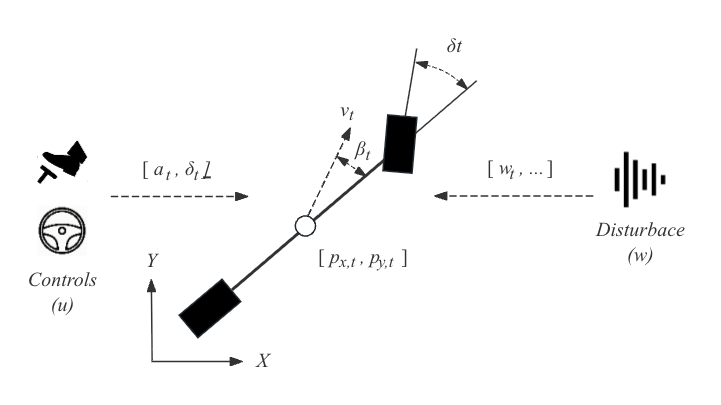
\includegraphics[width=0.7\textwidth]{figures/fig_vehicle_dynamics.png}
		\caption{Vehicle dynamics (kinematic bicycle model).}
		\label{fig1}
	\end{figure}
	
	\subsection{Problem Formulation}
	\label{subsec2}
	
	\subsubsection{Dynamic Model}
	To describe the vehicle motion at moderate to high speeds, we consider the kinematic bicycle model, which captures the essential geometric relationship between velocity, steering angle, and vehicle orientation without relying on tire force equations.
	
	\begin{equation} 
    s_{t+1} = f(s_t, u_t, w_t),\label{equ:dynamics}
	\end{equation}
	
	This equation describes the evolution of the vehicle from time step \(t\) to \(t+1\) under the nonlinear dynamics \(f(\cdot)\), which is defined by the kinematic bicycle model.
	
	The variables are defined as:
	\begin{enumerate}
		\item[i)] \( s_t \in \mathbb{R}^5 \) denotes the state vector, defined as:
		\begin{equation}
			s_t = \begin{bmatrix} p_{x,t} & p_{y,t} & \psi_t & v_t & \omega_t \end{bmatrix}^\top,
			\label{equ:sec2_state_vector}
		\end{equation}
		where \(t \in \{0,1,\dots,T\}\) are discrete time steps, \( p_x \) and \( p_y \) are the global position coordinates, \( \psi \) is the yaw angle, \( v \) is the longitudinal velocity, and \( \omega \) is the yaw rate.
		
		\item[ii)] \( u_t \in \mathbb{R}^2 \) denotes the control input, defined as:
		\begin{equation}
			u_t = \begin{bmatrix} a_t & \delta_t \end{bmatrix}^\top,
			\label{equ:sec2_control_vector}
		\end{equation}
		where \( a \) is the acceleration (positive for throttle, negative for braking) and \( \delta \) is the steering angle.
		
		\item[iii)] \( w_t \in \mathbb{R}^5 \) denotes the disturbance vector, defined as:
		\begin{equation}
			w_t = \begin{bmatrix} w_{x,t} & w_{y,t} & w_{\psi,t} & w_{v,t} & w_{\omega,t} \end{bmatrix}^\top,
			\label{equ:sec2_disturbance_vector}
		\end{equation}
		capturing the effect of exogenous uncertainties affecting the vehicle dynamics, including road irregularities, wind gusts, tire-road friction variations, and model mismatches between the nominal dynamics and the real system.
	\end{enumerate}
	
	\subsubsection{Optimization Objective}
	The objective is to track a reference trajectory while minimizing control effort:
	\begin{equation}
		\min_{\{u_t\}_{t=0}^{T-1}} \sum_{t=0}^{T-1} \left( \| s_t - s_t^{\text{ref}} \|_Q^2 + \|\Delta u_t\|_R^2 \right),
		\label{equ:sec2_tracking_objective}
	\end{equation}
	where \( \Delta u_t = u_t - u_{t-1} \).
	
	The weighting matrices are defined as:	
	\begin{equation}
		\begin{aligned}
			Q &= \operatorname{diag}(q_x,\; q_y,\; q_\psi,\; q_v,\; q_\omega) \in \mathbb{R}^{5 \times 5},\\
			R &= \operatorname{diag}(r_a,\; r_\delta) \in \mathbb{R}^{2 \times 2},
		\end{aligned}
		\label{equ:sec2_weight_matrices}
	\end{equation}
	with positive scalars \(q_x, q_y, q_\psi, q_v, q_\omega\) penalizing the tracking errors in position, yaw angle, longitudinal velocity, and yaw rate, respectively, and \(r_a, r_\delta\) penalizing changes in acceleration and steering angle. The squared Mahalanobis distance is defined as \(\|s\|_Q^2 = s^\top Q s\).
	
	\subsubsection{State Constraints}
	
	The vehicle must satisfy the following physical and safety limits at each time step. We retain a rectangular obstacle description for surrounding vehicles and represent the local drivable corridor by tangent half-spaces constructed from the road edges.
	
	\begin{enumerate}
		\item[i)] {Obstacle avoidance constraint (rectangular):}  
		Each surrounding obstacle \(j\) is represented by an axis-aligned rectangle
		\([
		x_j^{\min}, x_j^{\max}] \times [y_j^{\min}, y_j^{\max}]
		\).
		To preserve convexity and real-time tractability, obstacle avoidance is enforced through a preselected separating half-space
		\begin{equation}
			H_{\text{obs},j}
			\begin{bmatrix}
				p_{x,t} \\
				p_{y,t}
			\end{bmatrix}
			\le h_{\text{obs},j},
			\quad \forall j, \forall t \in \mathbb{Z}_{0:T}.
			\label{equ:sec2_obstacle_halfspace}
		\end{equation}
		The pair \((H_{\text{obs},j}, h_{\text{obs},j})\) is selected according to the relative position between the ego vehicle and the obstacle before solving the MPC problem, so that the vehicle is constrained to pass the obstacle on the chosen safe side with margin \(\eta > 0\).
		
		\item[ii)] {Road boundary constraint:}  
		At each prediction step, the local drivable corridor is approximated by two tangent lines constructed from the left and right road boundaries around the predicted reference point. Each tangent line is written in the standard form $ax+by=c$, where $(a,b)$ is the inward normal vector of the corresponding road edge and $c$ is determined by the boundary point through which that tangent line passes. Therefore, $(a_{1,t}, b_{1,t}, c_{1,t})$ and $(a_{2,t}, b_{2,t}, c_{2,t})$ denote the line coefficients associated with the left and right road boundaries at prediction step $t$, respectively. To write both boundary conditions in the same "$\le$" form required by the optimizer, we define
		\begin{equation}
			\begin{aligned}
				G_{\text{road},t} &=
				\begin{bmatrix}
					a_{1,t} & b_{1,t} \\
					-a_{2,t} & -b_{2,t}
				\end{bmatrix},
				\\
				h_{\text{road},t} &=
				\begin{bmatrix}
					c_{1,t} \\
					-c_{2,t}
				\end{bmatrix},
			\end{aligned}
			\label{equ:sec2_road_halfspace_matrices}
		\end{equation}
			so that the left-boundary constraint $a_{1,t} p_{x,t} + b_{1,t} p_{y,t} \le c_{1,t}$ and the right-boundary constraint $a_{2,t} p_{x,t} + b_{2,t} p_{y,t} \ge c_{2,t}$ are represented jointly. Then the vehicle position must satisfy
		\begin{equation}
			G_{\text{road},t}
			\begin{bmatrix}
				p_{x,t} \\
				p_{y,t}
			\end{bmatrix}
			\le h_{\text{road},t},
			\quad \forall t \in \mathbb{Z}_{0:T}.
			\label{equ:sec2_road_halfspace_constraint}
		\end{equation}
		This stagewise representation keeps the vehicle inside the local road corridor while adapting the admissible half-spaces along the curved track.
		
		\item[iii)] {Longitudinal velocity limits:}  
		The vehicle's forward speed is bounded by physical and legal limits:
		\begin{equation}
			v_{\min} \le v_t \le v_{\max}, \quad \forall t.
			\label{equ:sec2_velocity_limits}
		\end{equation}
		
		\item[iv)] {Acceleration limits:}  
		The longitudinal acceleration is bounded by actuator capabilities:
		\begin{equation}
			a_{\min} \le a_t \le a_{\max}, \quad \forall t.
			\label{equ:sec2_acceleration_limits}
		\end{equation}
		
		\item[v)] {Yaw rate limits:}  
		The yaw rate is constrained to prevent excessive rotation:
		\begin{equation}
			\omega_{\min} \le \omega_t \le \omega_{\max}, \quad \forall t.
			\label{equ:sec2_yaw_rate_limits}
		\end{equation}
	\end{enumerate}
	
	\subsubsection{Control Constraints}
	The control input set \( \mathcal{U} \subset \mathbb{R}^2 \) reflects actuator limits:
	\begin{equation}
		\mathcal{U} = \left\{ u = [a, \delta]^\top \in \mathbb{R}^2 \; \middle| \;
		a_{\min} \leq a \leq a_{\max},\ |\delta| \leq \delta_{\max}
		\right\}.
		\label{equ:sec2_control_input_set}
	\end{equation}
	
	The steering rate is additionally constrained by actuator dynamics:
	\begin{equation}
		|\delta_{t+1} - \delta_t| \leq \Delta\delta_{\max} \Delta t, \quad \forall t \in \mathbb{Z}_{0:T-2}.
		\label{equ:sec2_steering_rate_limit}
	\end{equation}
	
	\subsubsection{Nominal MPC Problem}
	The nominal MPC problem is formulated as:
	\begin{subequations}\label{equ:sec2_nominal_mpc}
	\begin{align}
		\min_{\{u_t\}_{t=0}^{T-1}} \quad & \sum_{t=0}^{T-1} \left( \| s_t - s_t^{\text{ref}} \|_Q^2 + \|\Delta u_t\|_R^2 \right) \nonumber \\
		\text{s.t.} \quad & s_{t+1} = f(s_t, u_t) + w_t, \quad \forall t \in \mathbb{Z}_{0:T-1}, \label{equ:sec2_nominal_dynamics} \\
		& s_0 = s_{\text{current}}, \label{equ:sec2_initial_condition} \\
		& v_{\min} \le v_t \le v_{\max}, \quad \forall t \in \mathbb{Z}_{0:T}, \label{equ:sec2_nominal_velocity_limits} \\
		& \omega_{\min} \le \omega_t \le \omega_{\max}, \quad \forall t \in \mathbb{Z}_{0:T}, \label{equ:sec2_nominal_yaw_rate_limits} \\
		& a_{\min} \le a_t \le a_{\max}, \quad \forall t \in \mathbb{Z}_{0:T-1}, \label{equ:sec2_nominal_acceleration_limits} \\
		& |\delta_t| \le \delta_{\max}, \quad \forall t \in \mathbb{Z}_{0:T-1}, \label{equ:sec2_nominal_steering_limits} \\
		& |\delta_{t+1} - \delta_t| \le \Delta\delta_{\max} \Delta t, \quad \forall t \in \mathbb{Z}_{0:T-2}, \label{equ:sec2_nominal_steering_rate_limit} \\
		& G_{\text{road},t} \begin{bmatrix} p_{x,t} \\ p_{y,t} \end{bmatrix} \le h_{\text{road},t}, \quad \forall t \in \mathbb{Z}_{0:T}, \label{equ:sec2_nominal_road_bounds} \\
		& H_{\text{obs},j} \begin{bmatrix} p_{x,t} \\ p_{y,t} \end{bmatrix} \le h_{\text{obs},j}, \quad \forall j, \forall t \in \mathbb{Z}_{0:T}. \label{equ:sec2_nominal_obstacle_bounds}
	\end{align}
	\end{subequations}
	
	Here, the obstacle constraint in \eqref{equ:sec2_nominal_obstacle_bounds} keeps the rectangular avoidance rule in a linear half-space form, while the road constraint in \eqref{equ:sec2_nominal_road_bounds} is represented by time-varying tangent half-spaces. This formulation serves as the baseline for the Koopman lifting and the tractable robust reformulations developed in the subsequent sections.
	
	\section{DATA-DRIVEN DEEP KOOPMAN MODEL}
	\label{sec3}
	
In this section, we will introduce the Koopman operator, the extended dynamic mode decomposition (EDMD) method, and a data-driven Deep Koopman model for autonomous vehicle obstacle avoidance.

\subsection{The Koopman Operator}

The Koopman operator was originally developed to describe the inherent properties of an uncontrolled nonlinear dynamical system through a linear evolutionary framework. With a slight modification, it can be adapted to controlled dynamical systems. In this paper, we consider a nonlinear dynamical system modeling autonomous vehicle dynamics. For clarity, we omit the noise term from system \eqref{equ:dynamics}, yielding the following deterministic form:
\begin{equation}
s_{t+1} = f(s_t, u_t), \label{equ:noiseless}
\end{equation}
Let $\mathbf{u}_t = (u_t, u_{t+1}, u_{t+2}, \ldots) \in \bar{\mathcal{U}}$, and define $\mathcal{G}$ as the left shift operator such that $\mathcal{G} \mathbf{u}_t = \mathbf{u}_{t+1}$. Here, $\bar{\mathcal{U}}$ denotes the space of all sequences $(u_0, u_1, u_2, \ldots)$ with $u_t \in \mathcal{U}$. We then define the Koopman operator for the dynamics on the extended state $[s, \mathbf{u}]$ as follows:
\begin{equation}
\mathcal{K} g(s_t, \mathbf{u}_t) = g(s_{t+1}, \mathbf{u}_{t+1}) = g(f(s_t, u_t), \mathcal{G} \mathbf{u}_t), \label{equ:extendedControl}
\end{equation}
where $\mathcal{K}: \mathcal{H} \to \mathcal{H}$ is the Koopman operator, $g: \mathcal{X} \times \bar{\mathcal{U}} \to \mathbb{R}^N$ is an observable function belonging to $\mathcal{H}$, and $\mathcal{H}$ is a Banach space. The Koopman operator $\mathcal{K}$ acts as a composition of $g$ with $f$. Notably, $\mathcal{K}$ is infinite-dimensional and linear, even when the dynamics $f(\cdot)$ is nonlinear. Due to this linearity, $\mathcal{K}$ admits a standard eigendecomposition:
\begin{equation}
\mathcal{K} \phi_j(s_t, \mathbf{u}_t) = \lambda_j \phi_j(s_t, \mathbf{u}_t), \quad j = 1, 2, \ldots, \label{equ:eig}
\end{equation}
where $\phi_j(s_t, \mathbf{u}_t)$ and $\lambda_j$ are the eigenfunction and associated eigenvalue of $\mathcal{K}$, respectively. A vector-valued observable $g$ can be expressed in terms of these eigenfunctions as:
\begin{equation}
g(s_t, \mathbf{u}_t) = (\mathcal{K}^t g)(s_0, \mathbf{u}_0) = \sum_{j=1}^{\infty} \lambda_j^t \phi_j(s_0, \mathbf{u}_0) \nu_j, \label{equ:eigenfunction}
\end{equation}
where $\mathcal{K}^t$ denotes the $t$-fold application of the Koopman operator, $\nu_j$ is the Koopman mode associated with eigenvalue $\lambda_j$, and $s_0$ is the initial state. 
\subsection{Extended Dynamic Mode Decomposition}

The extended dynamic mode decomposition (EDMD) is a method for obtaining a finite-dimensional approximation of the Koopman operator. EDMD employs a set of basis functions—such as radial basis functions (RBFs) with varying kernel centers and widths—to represent the observable functions, and uses the least squares method to compute a finite-dimensional approximation $\mathbf{K} \in \mathbb{R}^{N \times N}$ of $\mathcal{K}$. Note that it is generally infeasible to directly apply the least squares method to compute an approximation of the Koopman operator in finite time, because the extended state $[s, \mathbf{u}]$ is typically infinite-dimensional.

To obtain the finite-dimensional approximation $\mathbf{K}$, we choose the lifting functions $g_i$ for $i = 1, 2, \ldots, N$ in a specific form:
\begin{equation}
g_i(s_t, \mathbf{u}_t) = \psi_i(s_t) + h_i(\mathbf{u}_t), \label{equ:lifting}
\end{equation}
where $\psi_i: \mathcal{X} \to \mathbb{R}$ is generally nonlinear, while $h_i: \bar{\mathcal{U}} \to \mathbb{R}$ is linear. Without loss of generality, we assume the vector-valued observable function $g = [g_1, g_2, \ldots, g_N]^\top$ takes the form:
\begin{equation}
g(s_t, \mathbf{u}_t) = [\psi^\top(s_t), u_t^\top]^\top, \label{equ:liftingvector}
\end{equation}
where $\psi(s_t) = [\psi_1(s_t), \psi_2(s_t), \ldots, \psi_l(s_t)]^\top$ with $l = N - m$, and $u_t \in \mathbb{R}^m$ is the first component of the sequence $\mathbf{u}_t$. To avoid notational abuse, we consistently use $u_t$ to denote this first component throughout the paper. From \eqref{equ:extendedControl} and \eqref{equ:liftingvector}, we obtain:
\begin{equation}
\mathcal{K} g(s_t, \mathbf{u}_t) = \mathbf{K} [\psi^\top(s_t), u_t^\top]^\top + r(s_t, u_t), \label{equ:EDMD}
\end{equation}
where $r(s_t, u_t)$ is a residual term representing the discrepancy between the $N$-dimensional approximation of the observable space and the true lifted space of the Koopman operator. We determine $\mathbf{K}$ by minimizing the cost function $\| r(s_t, u_t) \|_2^2$. Since the future values of the control sequence are not needed for prediction, we can discard the last $m$ components of $[\psi^\top(s_{t+1}), u_{t+1}^\top]^\top$. Defining $\Psi(s_t) = [\psi^\top(s_t), u_t^\top]^\top$, we rewrite the observable dynamics governed by the Koopman operator as:
\begin{align}
\psi(s_{t+1}) &= \mathbf{A} \Psi(s_t), \notag \\
\tilde{s}_t &= C \psi(s_t), \label{equ:KoopmanOpertor}
\end{align}
where $\mathbf{A} = [A, B] \in \mathbb{R}^{l \times N}$ consists of $A \in \mathbb{R}^{l \times l}$ and $B \in \mathbb{R}^{l \times m}$. Here, $\mathbf{A}$ corresponds to the first $l$ rows of $\mathbf{K}$, $C \in \mathbb{R}^{n \times l}$ maps the lifted space back to the original state space, and $\tilde{s}_t \in \mathbb{R}^n$ is the reconstructed state approximating $s_t$. Consequently, the matrices $A$ and $B$ are obtained by solving the optimization problem:
\begin{equation}
\min_{A,B} \| r \|_2^2 = \min_{A,B} \sum_{t=0}^{T} \| \psi(s_{t+1}) - A \psi(s_t) - B u_t \|_2^2. \label{equ:koopmanconst}
\end{equation}
% The solution is given by:
% \begin{equation}
% [A, B] = S V^\top (V V^\top)^\dagger, \notag
% \end{equation}
% where $S = [\psi(s_1), \psi(s_2), \ldots, \psi(s_{T+1})]$, $V = [\Psi(s_0), \Psi(s_1), \ldots, \Psi(s_T)]$, and $\dagger$ denotes the Moore-Penrose pseudoinverse. The matrix $C$ is obtained by minimizing:
% \begin{equation}
% \min_{C} \sum_{t=0}^{T} \| s_t - C \psi(s_t) \|_2^2,
% \end{equation}
% which yields:
% \begin{equation}
% C = R D^\top (D D^\top)^\dagger, \notag
% \end{equation}
% with $R = [s_0, s_1, \ldots, s_T]$ and $D = [\psi(s_0), \psi(s_1), \ldots, \psi(s_T)]$. Notably, if the set of lifting functions $[\psi_1, \psi_2, \ldots, \psi_l]$ includes the state variables themselves—i.e., after a possible reordering, $\psi_i(s) = s_i$ for $i = 1, \ldots, n$—then $C = [I, 0]$, where $I$ is the $n \times n$ identity matrix. Further details on the computation of $A$ and $C$ can be found in the literature.

\subsection{The Deep Koopman Method}

Compared with the classic EDMD, the Deep Koopman model employs a deep neural network to generate the observable subspace of the Koopman operator. The proposed Deep Koopman model adopts an encoder-decoder architecture, where the encoder $\psi^e$ maps the system inputs to a lifted space, and the decoder $\psi^d$ reconstructs the original system states from the lifted features. The dynamical system is represented as:
\begin{align}
\psi^e(s_{t+1}, w^e) &= \widetilde{\mathbf{A}} \Phi(s_t, w^e, u_t), \label{equ:deep_koopman_encoder} \\
\tilde{s}_t &= \psi^d(\psi^e(s_t, w^e), w^d),  \label{equ:deep_koopman_decoder}
\end{align}
where $\widetilde{\mathbf{A}} = [\widetilde{A}, \widetilde{B}] \in \mathbb{R}^{l \times N}$, $\Phi(s_t, w^e, u_t) = [\psi^e(s_t, w^e)^\top, u_t^\top]^\top \in \mathbb{R}^N$, $\psi^e$ is the encoder with parameters $w^e$, and $\psi^d$ is the decoder with parameters $w^d$.

For the autonomous vehicle control problem, the state $s$ exhibits temporal dependencies. Therefore, a long short-term memory (LSTM) network is used to process sequential data within the encoder, i.e., $\psi^e(s, w^e)$, which lifts the original state $s$ to a higher-dimensional vector of observables. 

Let $K$ denote the sequence length of the state inputs to the encoder. The vector-valued observables are then given by the last hidden state of the LSTM:
\begin{equation}
\psi^e(s, w^e) = [s^\top, h_K^\top]^\top.  \label{equ:lstm_observables}
\end{equation}

The decoder $\psi^d$ is constructed using a feed-forward neural network consisting of $K'$ fully connected layers, which recover the original state from the higher-dimensional observables. The output of any hidden layer $k \in \{1, 2, \ldots, K'\}$ is expressed as:
\begin{equation}
h_k^d = \sigma_k^d (W_k^d h_{k-1}^d + b_k^d).  \label{equ:decoder_hidden}
\end{equation}

The predicted state is obtained from the output of the decoder's final layer:
\begin{equation}
\tilde{s}_t = \psi^d(\psi^e(s_t, w^e), w^d) = \sigma(W_{K'}^d h_{K'-1}^d + b_{K'}^d). \label{equ:decoder_output}
\end{equation}

Then, the parameters $W$ and $b$ are learned by optimizing a fixed loss function during training. To accurately approximate autonomous vehicle dynamics over a longer time horizon, a multi-step prediction error is considered instead of a single-step error. To formulate the multi-step loss function, we first present the state prediction over an $M$-step interval:

\begin{equation}
s_{t+M} = \psi^d( \widetilde{A}^M \Phi(s_t, w^e, u_t), w^d ) + r(s, M),  \label{equ:multi_step_prediction}
\end{equation}
where $\widetilde{A}^M \Phi(s_t, w^e, u_t)$ represents the $M$-step ahead lifted state starting from $s_t$, given by:
\begin{align}
\widetilde{A}^M \Phi(s_t, w^e, u_t) &= \psi^e(s_{t+M}, w^e) \nonumber \\
&= \widetilde{A} \psi^e(s_{t+M-1}, w^e) + \widetilde{B} u_{t+M-1} \nonumber \\
&= \widetilde{A}^M \psi^e(s_t, w^e) + \sum_{s=1}^{M} \widetilde{A}^{s-1} \widetilde{B} u_{t+M-s}. \label{equ:lifted_multistep}
\end{align}

The main components of the loss function over $M$ time steps are defined as:
\begin{align}
L_1 &= \frac{1}{M} \sum_{s=1}^{M} \| s_{t+s} - \psi^d( \widetilde{A}^s \Phi(s_t, w^e, u_t), w^d ) \|_2^2, \label{equ:loss_prediction} \\
L_2 &= \frac{1}{M} \sum_{s=1}^{M} \| \psi^e(s_{t+s}, w^e) - \widetilde{A}^s \Phi(s_t, w^e, u_t) \|_2^2, \label{equ:loss_lifted} \\
L_3 &= \frac{1}{M} \sum_{s=1}^{M} \| s_s - \psi^d( \psi^e(s_s, w^e), w^d ) \|_2^2, \label{equ:loss_reconstruction}
\end{align}
where $L_1$ denotes the prediction error, $L_2$ the prediction error in the lifted observable space, and $L_3$ the reconstruction error. Using these definitions, the overall optimization problem is formulated as:
\begin{equation}
\min_{w^e, w^d, \widetilde{A}, \widetilde{B}} L = \alpha_1 L_1 + \alpha_2 L_2 + \alpha_3 L_3 + \alpha_4 \| w^e \|_2^2 + \alpha_5 \| w^d \|_2^2,  \label{equ:total_loss}
\end{equation}
where $\alpha_i$, $i = 1, 2, \ldots, 5$, are weight parameters, and the last two terms serve as regularization terms to prevent overfitting.

After training the Deep Koopman model, the approximated dynamics for the autonomous vehicle are given by:
\begin{align}
\psi^e(s_{t+1}, w^e) &= \widetilde{A} \psi^e(s_t, w^e) + \widetilde{B} u_t,  \label{equ:trained_encoder} \\
\tilde{s}_t &= \psi^d( \psi^e(s_t, w^e), w^d ). \label{equ:trained_decoder}
\end{align}

\begin{figure*}[t]
	\centering
	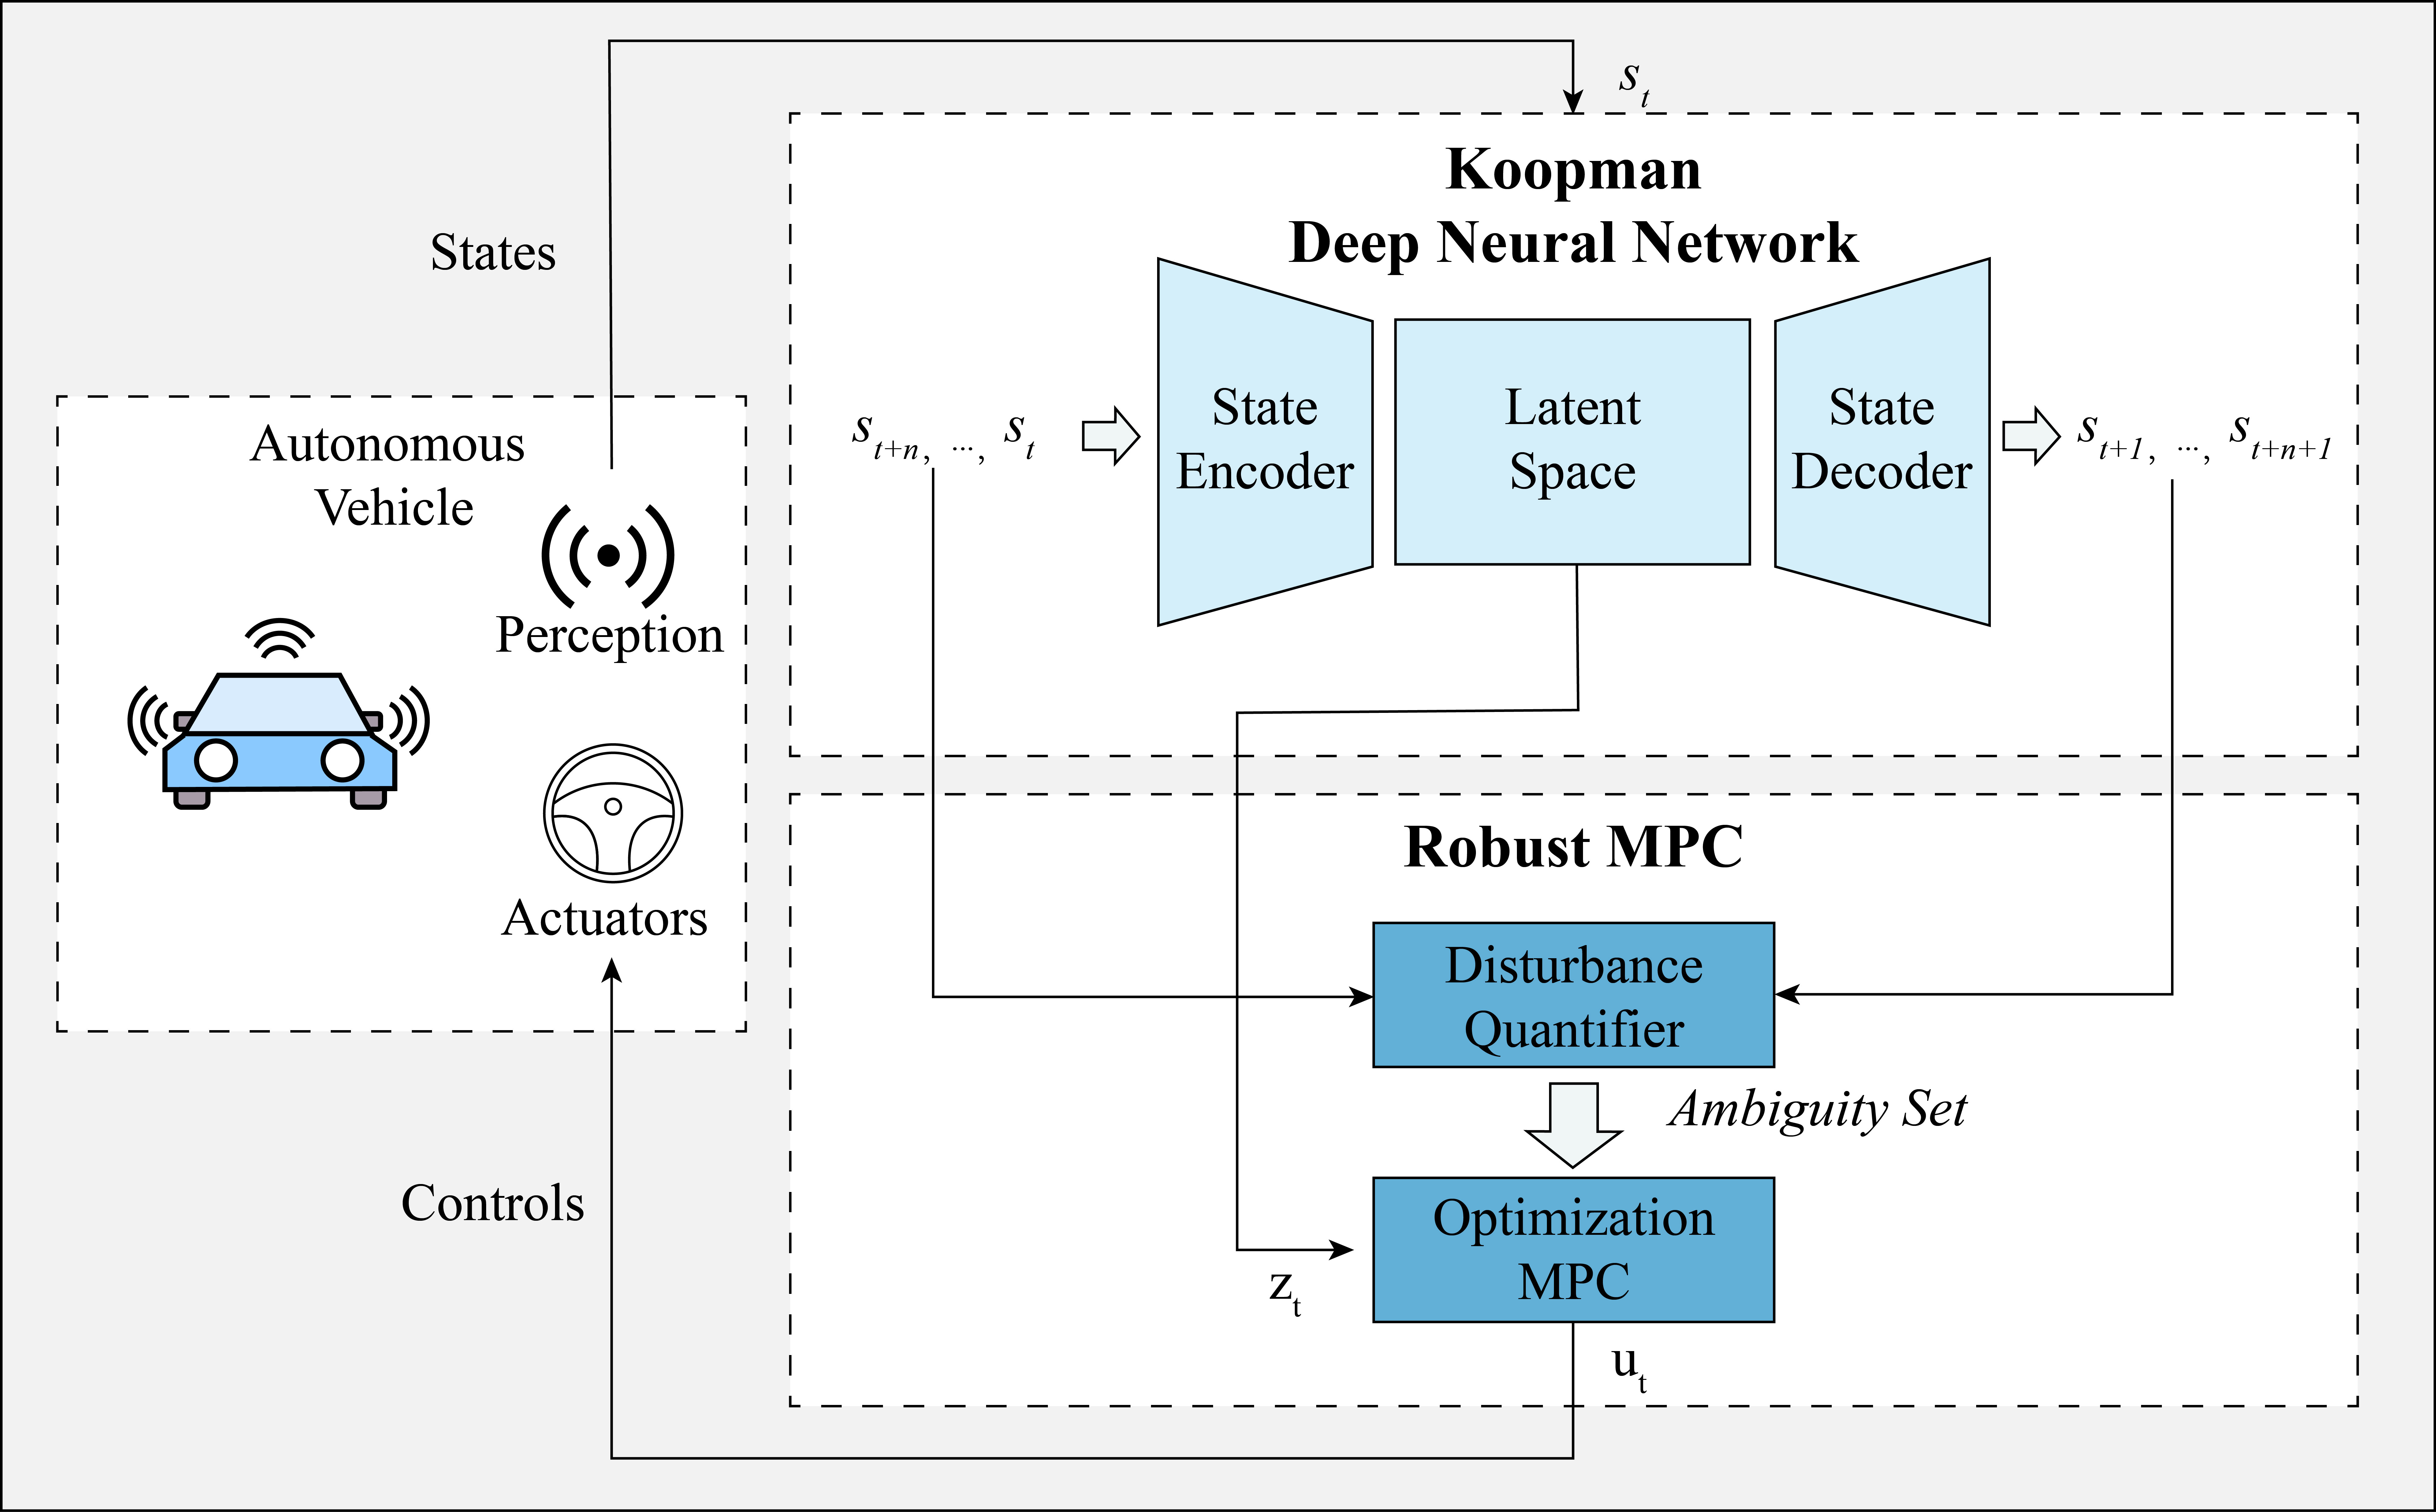
\includegraphics[width=0.8\linewidth]{figures/koopman_architecture.jpg}
	\caption{Overall architecture of the proposed Koopman-based robust MPC framework. The measured vehicle states are lifted to a latent space through a deep Koopman encoder-decoder model. The latent dynamics and disturbance quantification are then integrated into a robust MPC optimization with a Wasserstein ambiguity set, and the resulting control input is fed back to the autonomous vehicle.}
	\label{fig:koopman_architecture}
\end{figure*}

\subsection{Distributionally Robust Obstacle Avoidance}

To ensure safe obstacle avoidance under uncertain disturbances, we impose a distributionally robust chance constraint on the safety margin over the entire prediction horizon. For this purpose, after training the Deep Koopman model, we obtain the encoder $\psi^e$, the decoder $\psi^d$, and the linear dynamics matrices $\widetilde{A}$ and $\widetilde{B}$. The lifted state evolves according to:
\begin{equation}
z_{t+1} = \widetilde{A} z_t + \widetilde{B} u_t + \hat{w}(s_t, u_t, w_t), \quad z_t = \psi^e(s_t), \label{equ:lifted_dynamics}
\end{equation}
and the physical state is recovered via $s_t = \psi^d(z_t)$, where $\hat{w}(\cdot)$ captures the combined effect of model mismatch and external disturbances. In the Koopman lifting design, the first five components of the latent state $z_t$ correspond directly to the original physical state:
\begin{equation}
z_t = [p_{x,t}, p_{y,t}, \psi_t, v_t, \omega_t, \ldots]^\top. \label{equ:latent_state}
\end{equation}

We treat the entire combined disturbance sequence over the prediction horizon as a single random vector. Define:
\begin{equation}
\hat{\mathbf{w}} = \begin{bmatrix} \hat{w}_0 \\ \hat{w}_1 \\ \vdots \\ \hat{w}_{T-1} \end{bmatrix} \in \mathbb{R}^{n_z T}, \label{equ:def_hatw}
\end{equation}
where $\hat{w}_t = \hat{w}_t(s_t,u_t,w_t)$ is the combined disturbance at time $t$. Given $N$ independent historical trajectories $\{\hat{\mathbf{w}}^{(i)}\}_{i=1}^N$, the empirical distribution is $\hat{\mathbb{P}}_N = \frac{1}{N}\sum_{i=1}^N \delta_{\hat{\mathbf{w}}^{(i)}}$. We use the first-order Wasserstein distance induced by a ground norm $\|\cdot\|$ on $\mathbb{R}^{n_z T}$, with dual norm $\|\cdot\|_*$. Since the disturbance generator used in the simulations is a Gaussian mixture with unbounded support, the ambiguity set is defined over distributions with finite first moment:
\begin{equation}
\mathcal{D} = \left\{ \mathbb{P} \in \mathcal{P}_1(\mathbb{R}^{n_z T}) \;\middle|\; W_1(\mathbb{P}, \hat{\mathbb{P}}_N) \le \theta \right\}, \label{equ:wass_ambiguity}
\end{equation}
where $\mathcal{P}_1$ denotes the set of distributions with finite first moment. The ground norm and the units of $\theta$ must be reported with the experimental settings.

Define the linear projection matrices as follows:
\begin{equation}
D = \begin{bmatrix} 1 & 0 & \cdots & 0 \\ 0 & 1 & \cdots & 0 \end{bmatrix}, \quad 
E = \begin{bmatrix} 0 & 0 & 0 & 1 & 0 & \cdots & 0 \end{bmatrix}, \quad 
F = \begin{bmatrix} 0 & 0 & 0 & 0 & 1 & \cdots & 0 \end{bmatrix}. \label{equ:projection_matrices}
\end{equation}
Thus, the position, velocity, and yaw rate can be extracted as:
\begin{equation}
D z_t = \begin{bmatrix} p_{x,t} \\ p_{y,t} \end{bmatrix}, \quad E z_t = v_t, \quad F z_t = \omega_t, \quad C_y z_t = \begin{bmatrix} v_t \\ \omega_t \end{bmatrix}. \label{equ:state_extraction}
\end{equation}

Let $l_{j,t}(s_t, \hat{w}_t)$ denote the safety margin for obstacle $j$ at time $t$:
\begin{equation}
l_{j,t}(s_t, \hat{w}_t) = H_{\text{obs},j} D z_t - h_{\text{obs},j} \leq 0. \label{equ:safety_margin}
\end{equation}
Then, distributionally robust obstacle avoidance is enforced via the following constraints:
\begin{equation}
\inf_{\mathbb{P} \in \mathcal{D}} \Pr_{\mathbb{P}}\bigl( l_{j,t}(s_t, \hat{w}_t) \le 0 \bigr) \ge 1 - \epsilon, \quad \forall j,\; \forall t = 0,\dots,T-1. \label{equ:per_step_chance}
\end{equation}
Here $\epsilon \in (0,1)$ is a small risk parameter (e.g., $0.05$). Because the ambiguity set $\mathcal{D}$ contains distributions of the entire trajectory $\hat{\mathbf{w}}$, the marginal distribution of $\hat{w}_t$ is not fixed. Constraint \eqref{equ:per_step_chance} guarantees that for each time step, even under the worst-case joint distribution within $\mathcal{D}$, the probability of violating safety at that step is at most $\epsilon$.

Under this setting, the stage cost is defined as:
\begin{equation}
c(z_t, u_t) = \| C_y z_t - y_t^{\text{ref}} \|_Q^2 + \|\Delta u_t\|_R^2, \label{equ:stage_cost}
\end{equation}
where $Q = \text{diag}(Q_v, Q_\omega)$ and $R = \text{diag}(R_a, R_\delta)$.

Over the horizon, the tracking objective is written as
\begin{equation}
\sum_{t=0}^{T-1} \left\| C_y z_t - y_t^{\text{ref}} \right\|_{Q}^2. \label{equ:tracking_error}
\end{equation}

The control smoothness term is
\begin{equation}
\sum_{t=0}^{T-1} \left\| u_t - u_{t-1} \right\|_{R}^2. \label{equ:smoothness_penalty}
\end{equation}

Hence, the total stage-wise cost is
\begin{equation}
J = \sum_{t=0}^{T-1}\!\left( \left\| C_y z_t - y_t^{\text{ref}} \right\|_{Q}^2 + \left\| u_t - u_{t-1} \right\|_{R}^2 \right). \label{equ:total_cost}
\end{equation}

The optimization uses the empirical expected tracking cost over the available historical disturbance trajectories, as defined in Section~5.1. The Wasserstein ambiguity set is used to impose distributionally robust safety constraints; the quadratic tracking objective is not a worst-case expectation over that set.

Following the advisor's latest guidance, this manuscript version directly develops the tractable reformulation from per-step chance constraints and lifted dynamics.


\section{Tractable Reformulation}

To ensure safe obstacle avoidance under uncertain disturbances, we impose per-step distributionally robust chance constraints as in (\ref{equ:per_step_chance}). The tracking objective is the empirical expected cost, while the Wasserstein ambiguity set is used in the safety constraints.

\subsection{Empirical tracking objective under unbounded disturbances}

Let $\hat{\mathbf{w}} = [\hat{w}_0^\top,\hat{w}_1^\top,\dots,\hat{w}_{T-1}^\top]^\top \in \mathbb{R}^{n_z T}$ denote the combined disturbance trajectory over the prediction horizon. For a fixed control sequence $\{u_t\}_{t=0}^{T-1}$ and initial lifted state $z_0 = \psi^e(s_{\text{current}})$, the total cost defined in (\ref{equ:total_cost}) is
\begin{equation}
J(\hat{\mathbf{w}}) = \sum_{t=0}^{T-1}\left( \|C_y z_t - y_t^{\text{ref}}\|_Q^2 + \|u_t - u_{t-1}\|_R^2 \right),
\end{equation}
where the lifted states evolve according to (\ref{equ:lifted_dynamics}):
\begin{equation}
z_{t+1} = A z_t + B u_t + \hat{w}_t, \qquad t=0,\dots,T-1.
\end{equation}
Because the dynamics are affine, $J$ is a convex quadratic function of $\hat{\mathbf{w}}$ when the cost weights are positive semidefinite. Over an unbounded support, however, a nonconstant quadratic loss generally has an infinite worst-case expectation over a positive-radius $W_1$ ball: a small amount of probability mass can be transported arbitrarily far while incurring only a linear transportation cost. The finite-first-moment assumption defining $\mathcal{D}$ does not preclude such distributions. Accordingly, the objective used here is the empirical expected tracking cost, not the worst-case expected cost:
\begin{equation}
J_{\mathrm{emp}}(\{u_t\}) := \frac{1}{N}\sum_{i=1}^{N}J(\hat{\mathbf{w}}^{(i)};\{u_t\}).
\label{eq:empirical_objective}
\end{equation}

\subsection{Conservative reformulation of distributionally robust chance constraints}

For each obstacle $j$ and time step $t$, the safety constraint (3.30) is
\begin{equation}
\inf_{\mathbb{P}\in\mathcal{D}} \Pr_{\mathbb{P}}\bigl( H_{\text{obs},j}D z_t - h_{\text{obs},j} \le 0 \bigr) \ge 1-\epsilon,
\qquad \epsilon\in(0,1). \label{eq:safety}
\end{equation}

Define the safety residual $g_{j,t}(\hat{\mathbf{w}}) := H_{\text{obs},j}D z_t-h_{\text{obs},j}$, so that safety is the event $g_{j,t}(\hat{\mathbf{w}})\le0$.

Using the lifted dynamics (\ref{equ:lifted_dynamics}), $z_t$ is an affine function of $\hat{\mathbf{w}}$:
\begin{equation}
z_t = A^t z_0 + \sum_{k=0}^{t-1} A^{t-1-k} B u_k \;+\; \sum_{k=0}^{t-1} A^{t-1-k} \hat{w}_k.
\end{equation}

Define the constant row vector (for fixed $j,t$)
\begin{equation}
c_{j,t}^\top \;:=\; H_{\text{obs},j}D \bigl[ A^{t-1},\; A^{t-2},\; \dots,\; I,\; 0,\; \dots,\; 0 \bigr] \in \mathbb{R}^{1\times n_z T},
\end{equation}
and the deterministic term
\begin{equation}
d_{j,t} \;:=\; h_{\text{obs},j} - H_{\text{obs},j}D\left( A^t z_0 + \sum_{k=0}^{t-1} A^{t-1-k} B u_k \right),
\end{equation}
which depends linearly on the control sequence. Then
\begin{equation}
H_{\text{obs},j}D z_t - h_{\text{obs},j} = c_{j,t}^\top \hat{\mathbf{w}} - d_{j,t},
\end{equation}
and therefore
\begin{equation}
\ell_{j,t}(\hat{\mathbf{w}}) = \bigl( c_{j,t}^\top \hat{\mathbf{w}} - d_{j,t} \bigr)_+
= \max\{0,\; c_{j,t}^\top \hat{\mathbf{w}} - d_{j,t}\}.
\end{equation}

For a fixed margin parameter $\delta_{j,t}>0$, define the shifted hinge loss $\ell_{j,t}^{\delta}(\hat{\mathbf{w}}):=(g_{j,t}(\hat{\mathbf{w}})+\delta_{j,t})_+$. Pointwise, $\mathbf{1}_{\{g_{j,t}>0\}}\le \ell_{j,t}^{\delta}/\delta_{j,t}$, so controlling its worst-case expectation gives a sufficient, generally conservative condition for \eqref{eq:safety}.

\begin{theorem}
\label{thm:cc}
Let $\xi\in\mathbb{R}^{m}$, let $\hat{\mathbb{P}}_N=N^{-1}\sum_{i=1}^N\delta_{\hat{\xi}_i}$, and define a $W_1$ ball of radius $\theta$ over $\mathcal{P}_1(\mathbb{R}^{m})$ using the ground norm $\|\cdot\|$. For $g(\xi)=c^\top\xi-d$ and fixed $\delta>0$, the worst-case expected shifted hinge is
\begin{equation}
\sup_{\mathbb{P}:W_1(\mathbb{P},\hat{\mathbb{P}}_N)\le\theta}
\mathbb{E}^{\mathbb{P}}[(g(\xi)+\delta)_+]
=\frac{1}{N}\sum_{i=1}^N(c^\top\hat{\xi}_i-d+\delta)_+ + \theta\|c\|_*.
\label{eq:worst_case_hinge}
\end{equation}
Consequently, the following condition is sufficient for $\sup_{\mathbb{P}\in\mathcal{D}}\mathbb{P}(g(\xi)>0)\le\epsilon$:
\begin{equation}
\frac{1}{N}\sum_{i=1}^N(c^\top\hat{\xi}_i-d+\delta)_+ + \theta\|c\|_* \le \delta\epsilon.
\label{eq:drcc_sufficient}
\end{equation}
\end{theorem}

\begin{proof}
The shifted hinge is $\|c\|_*$-Lipschitz. In the Wasserstein dual representation, multipliers below $\|c\|_*$ give an infinite inner supremum on $\mathbb{R}^m$, while for multipliers at least $\|c\|_*$ the inner supremum equals the hinge value at the empirical sample. Minimizing the dual objective therefore gives \eqref{eq:worst_case_hinge}. Pointwise, $\mathbf{1}_{\{g(\xi)>0\}}\le (g(\xi)+\delta)_+/\delta$; taking expectations and the supremum over $\mathcal{D}$ proves \eqref{eq:drcc_sufficient}.
\end{proof}

Applying Theorem~\ref{thm:cc} with $c=c_{j,t}$, $d=d_{j,t}$, and a fixed $\delta_{j,t}>0$, we obtain for each obstacle $j$ and time $t$ the following linear sufficient conditions, where $s_{j,t,i}$ are epigraph variables:
\begin{align}
\frac{1}{N}\sum_{i=1}^{N} s_{j,t,i} + \theta\|c_{j,t}\|_* &\le \delta_{j,t}\epsilon, \label{eq:ccfinal1} \\
s_{j,t,i} &\ge c_{j,t}^\top \hat{\mathbf{w}}^{(i)} - d_{j,t} + \delta_{j,t}, \quad s_{j,t,i}\ge0. \label{eq:ccfinal2}
\end{align}
The values $\delta_{j,t}$ are fixed design parameters, not optimization variables. Since $c_{j,t}$ is fixed and $d_{j,t}$ is affine in the control sequence, these constraints are affine in the decision variables.

\subsection{Distributionally robust MPC problem reformulation}

Combining the cost reformulation and the chance‑constraint reformulation \eqref{eq:ccfinal1}–\eqref{eq:ccfinal2}, we obtain the following convex quadratic program:

\begin{align}
\min_{\{u_t,z_t\},\;\{s_{j,t,i}\}} 
&\quad J_{\mathrm{emp}}(\{u_t\}) \nonumber \\
\text{s.t.} 
&\quad z_{t+1} = A z_t + B u_t + \hat{w}_t,\quad u_t = K z_t + v_t,\quad z_0 = \psi^e(s_{\text{current}}), \nonumber \\
&\quad v_{\min} \le E z_t \le v_{\max},\quad \forall t, \nonumber \\
&\quad \omega_{\min} \le F z_t \le \omega_{\max},\quad \forall t, \nonumber \\
&\quad a_{\min} \le a_t \le a_{\max},\quad \forall t, \nonumber \\
&\quad |\delta_t| \le \delta_{\max},\quad \forall t, \nonumber \\
&\quad |\delta_{t+1} - \delta_t| \le \Delta\delta_{\max}\Delta t,\quad \forall t, \nonumber \\
&\quad G_{\text{road},t} D z_t \le h_{\text{road},t},\quad \forall t, \nonumber \\
&\quad \frac{1}{N}\sum_{i=1}^{N}s_{j,t,i} + \theta\|c_{j,t}\|_* \le \delta_{j,t}\epsilon,\quad \forall j,\forall t, \nonumber \\
&\quad s_{j,t,i} \ge 0,\quad s_{j,t,i} \ge c_{j,t}^\top \hat{\mathbf{w}}^{(i)} - d_{j,t} + \delta_{j,t},\quad \forall j,t,i. \label{eq:final}
\end{align}

For fixed $\delta_{j,t}$, all constraints in \eqref{eq:final} are affine and the empirical objective is quadratic; hence the problem retains its convex QP structure. The safety constraints are conservative sufficient conditions for the per-step distributionally robust chance constraints. The empirical objective is not claimed to minimize the worst-case expected quadratic cost over the unbounded Wasserstein ambiguity set.

	\section{SIMULATION AND NUMERICAL RESULTS}
	\label{sec:simulation}
	
	This section evaluates the proposed Koopman-based distributionally robust MPC (K-DRMPC) in closed-loop simulation to assess whether distributionally robust constraints improve robustness under distribution shift while preserving nominal tracking performance.
	The evaluation examines complementary dimensions: (i) nominal performance parity under in-distribution disturbances relative to non-robust K-MPC, (ii) robustness gains under distribution shift in safety-related indicators such as success rate and lateral error percentiles, and (iii) the trade-off between safety, performance, and computational overhead as the parameters $(\theta,\epsilon)$ are tuned. The evidence chain is organized around reproducibility protocol, failure mechanism analysis, distribution-shift robustness studies, and sensitivity studies.
	
	\subsection{Experimental Setup and Compared Methods}
	\label{subsec:protocol}
	
	Experiments are performed on the Serpentine track for closed-loop tracking testing with boundary termination conditions. A run terminates early if the boundary condition is violated (e.g., $|e_y| \ge 10.0$ m), or when the maximum simulation steps are reached. In the quadratic-program implementation, yaw references across each prediction horizon are unwrapped and shifted by an integer multiple of $2\pi$ to the equivalent branch nearest the current yaw, preventing artificial discontinuities at the $-\pi/\pi$ branch cut.
	
	Compared methods. Two configurations are evaluated to isolate the effect of distributionally robust constraints:
	\begin{enumerate}
		\item[i)] K-MPC (Non-Robust): Standard Koopman MPC with deterministic obstacle avoidance constraints only. Constraint \eqref{equ:sec2_nominal_obstacle_bounds} applies without the distributionally robust chance-constraint safety layer.
		\item[ii)] K-DRMPC (Robust): Full distributionally robust formulation in Section~5, namely problem \eqref{eq:final}, incorporating the Wasserstein ambiguity set with radius $\theta > 0$ and risk level $\epsilon \in (0,1)$.
	\end{enumerate}

	Disturbance-shift protocol. In this study, the disturbance is modeled as an unknown additive term in the lifted dynamics, and no parametric family (e.g., Gaussian or Laplace) is assumed for the true distribution. Three disturbance settings are tested to create distributional shifts relative to the training data:
	\begin{enumerate}
		\item[i)] Setting A (Nominal, $\times 1.0$): The disturbance distribution matches the training set (empirical distribution $\hat{\mathbb{P}}_N$). K-MPC and K-DRMPC are expected to exhibit similar nominal performance.
		\item[ii)] Setting B (Moderate Shift, $\times 1.5$): The disturbance magnitude increases moderately. The true distribution departs from $\hat{\mathbb{P}}_N$ but may still lie within a properly chosen Wasserstein ball. K-DRMPC is expected to maintain safety better than K-MPC.
		\item[iii)] Setting C (Large Shift, $\times 2.0$): A severe out-of-distribution disturbance is applied. K-DRMPC with larger $\theta$ should retain stronger safety guarantees, while K-MPC is more likely to fail.
	\end{enumerate}
	
	Vehicle model and sampling. The controlled plant is a kinematic bicycle model with state
	$s_t=[p_{x,t},p_{y,t},\psi_t,v_t,\omega_t]^\top$ and input $u_t=[a_t,\delta_t]^\top$.
	The sampling time is $\Delta t=0.1$~s and the wheelbase is $L=2.6$~m.
	The MPC prediction horizon is set to $T=20$ steps (2.0 s).
	The Koopman latent dimension is $n_z=32$. 
	
	Controller and solver settings. Table~\ref{tab:sim_params} summarizes the key parameters used in simulation and optimization.
	
	\begin{table}[htbp]
		\centering
		\caption{Simulation and optimization parameters (shared by K-MPC and K-DRMPC).}
		\label{tab:sim_params}
		\scriptsize
		\setlength{\tabcolsep}{3pt}
		\begin{tabularx}{\columnwidth}{>{\raggedright\arraybackslash}X c c}
			\toprule
			\textbf{Item} & \textbf{Symbol} & \textbf{Value} \\
			\midrule
			Sampling time & $\Delta t$ & 0.1 s \\
			Wheelbase & $L$ & 2.6 m\\
			Prediction horizon & $T$ & 20 steps\\
			Latent dimension & $n_z$ & 32 \\
			Speed limits & $[v_{\min},v_{\max}]$ & [0.0, 4.0] m/s \\
			Acceleration limits & $[a_{\min},a_{\max}]$ & [-0.6, 0.5] m/s\^2 \\
			Steering limit & $\delta_{\max}$ & 12.0 deg \\
			Steering-rate limit & $\dot{\delta}_{\max}$ & 2.00 rad/s \\
			Geometric safety margin & $\eta$ & 0.50 m \\
			Solver & -- & IPOPT \\[2pt]
			\midrule
			\multicolumn{3}{l}{\textbf{Non-Robust (K-MPC) specific:}} \\
			Obstacle avoidance & \eqref{equ:sec2_nominal_obstacle_bounds} & Deterministic inequality \\
			\midrule
			\multicolumn{3}{l}{\textbf{Robust (K-DRMPC) specific:}} \\
			Wasserstein ground norm & $\|\cdot\|$ & Euclidean after coordinate-wise residual standardization \\
			Wasserstein radius & $\theta$ & 0.01 (pilot setting) \\
			Chance-constraint risk level & $\epsilon$ & 0.10 (pilot setting) \\
			Shifted-hinge margin & $\delta_{j,t}$ & 0.5 m (pilot setting) \\
			Obstacle avoidance & \eqref{eq:final} & Conservative sufficient condition \\
			\bottomrule
		\end{tabularx}
	\end{table}
	The listed robust parameters are pilot settings; their final values will be selected after the sensitivity and repeated-run experiments with the revised formulation.
	
	Metrics and statistical protocol. Table~\ref{tab:metrics_protocol} summarizes all reported metrics and their statistical definitions.
	
	\begin{table}[htbp]
		\centering
		\caption{Metrics and statistical protocol used in Section 6.}
		\label{tab:metrics_protocol}
		\scriptsize
		\setlength{\tabcolsep}{2pt}
		\begin{tabularx}{\columnwidth}{>{\raggedright\arraybackslash}p{0.20\columnwidth} >{\raggedright\arraybackslash}p{0.31\columnwidth} >{\raggedright\arraybackslash}X}
			\toprule
			\textbf{Category} & \textbf{Metric} & \textbf{Definition / Statistic} \\
			\midrule
			Tracking & Lateral error $|e_y|$ & Mean, 95th percentile, and maximum over closed-loop steps. \\
			Tracking & Heading error $|e_\psi|$ & Mean, 95th percentile, and maximum over closed-loop steps. \\
			Safety & Completion status & Binary indicator (completed / terminated). \\
			Safety & Minimum safety margin $m_{\min}$ & With signed margin $m_t = h_{\mathrm{obs},j} - H_{\mathrm{obs},j}Dz_t$, report $m_{\min}=\min_t m_t$ (larger is safer; negative indicates violation). \\
			Safety & Safety-margin quantile $m_{\mathrm{P05}}$ & 5th percentile of $\{m_t\}$ over closed-loop steps, used to reduce sensitivity to single-step outliers. \\
			Safety & Crash step / crash time & First step and corresponding time when boundary/safety violation occurs. \\
			Safety & Violation rate & Ratio of violating steps to total simulated steps. \\
			Computational & Solve time per MPC step & Mean solve time (ms) over all optimization calls. \\
			Computational & Solve-time percentiles & P50, P95, and P99 of solve time (ms). \\
			Stability & Longest out-of-band interval & Maximum consecutive duration with $|e_y|>2$ m (in steps or seconds). \\
			\bottomrule
		\end{tabularx}
	\end{table}
	
	For obstacle-avoidance evaluation, the signed safety margin at time step $t$ is defined as
	\begin{equation}
	\label{equ:signed_safety_margin}
	m_t := h_{\mathrm{obs},j} - H_{\mathrm{obs},j} D z_t,
	\end{equation}
	where $m_t>0$ indicates safe separation, $m_t=0$ indicates boundary contact, and $m_t<0$ indicates violation. At the trajectory level, we report the minimum safety margin
	\begin{equation}
	\label{equ:min_safety_margin}
	m_{\min}:=\min_t m_t,
	\end{equation}
	as a single scalar safety indicator, together with the 5th-percentile statistic $m_{\mathrm{P05}}$ to reduce sensitivity to single-step outliers.
	
	When repeated experiments are available, all scalar metrics should additionally report mean$\pm$std and confidence intervals.
	In the following subsection, safety-margin statistics are reported together with completion status to make the safety-performance trade-off explicit.
	
	\subsection{Simulation Results and Sensitivity Analysis}
	\label{subsec:closed_loop_results}
	
	Figure~\ref{fig:traj_main} first provides a geometric view of the closed-loop behavior in the primary scenario. The robust controller follows a smoother path around obstacle clusters and maintains larger boundary clearance at turning segments, while the non-robust controller shows visibly larger path excursions in high-curvature regions. This qualitative contrast is consistent with the quantitative evidence reported later in Table~\ref{tab:main_results} and supports the interpretation that robustness mainly improves feasibility and tail behavior under distribution shift.
	More specifically, the primary experimental differences can be summarized along three dimensions. First, reliability is the dominant separator: Settings A and B do not distinguish the controllers in terms of completion, but under the severe shift of Setting C the comparison changes from nominal parity to a clear feasibility gap, indicating that the main value of the robust formulation lies in preserving task completion under mismatch rather than merely improving benign-regime averages. Second, the robust advantage is concentrated in the error tails. Even when mean tracking differences remain moderate, K-DRMPC consistently reduces large excursions, especially in the P95 lateral and heading errors, which explains why the geometric trajectories appear visibly smoother in the most demanding regions. Third, this robustness gain is not free: it is achieved at a moderate but stable computational surcharge, meaning that the method should be interpreted as exchanging additional solve time for substantially improved mismatch tolerance. For safety-critical deployment, this trade-off is favorable because failure prevention under distribution shift is more decision-relevant than small nominal-speed differences.

	\begin{figure}[htbp]
		\centering
		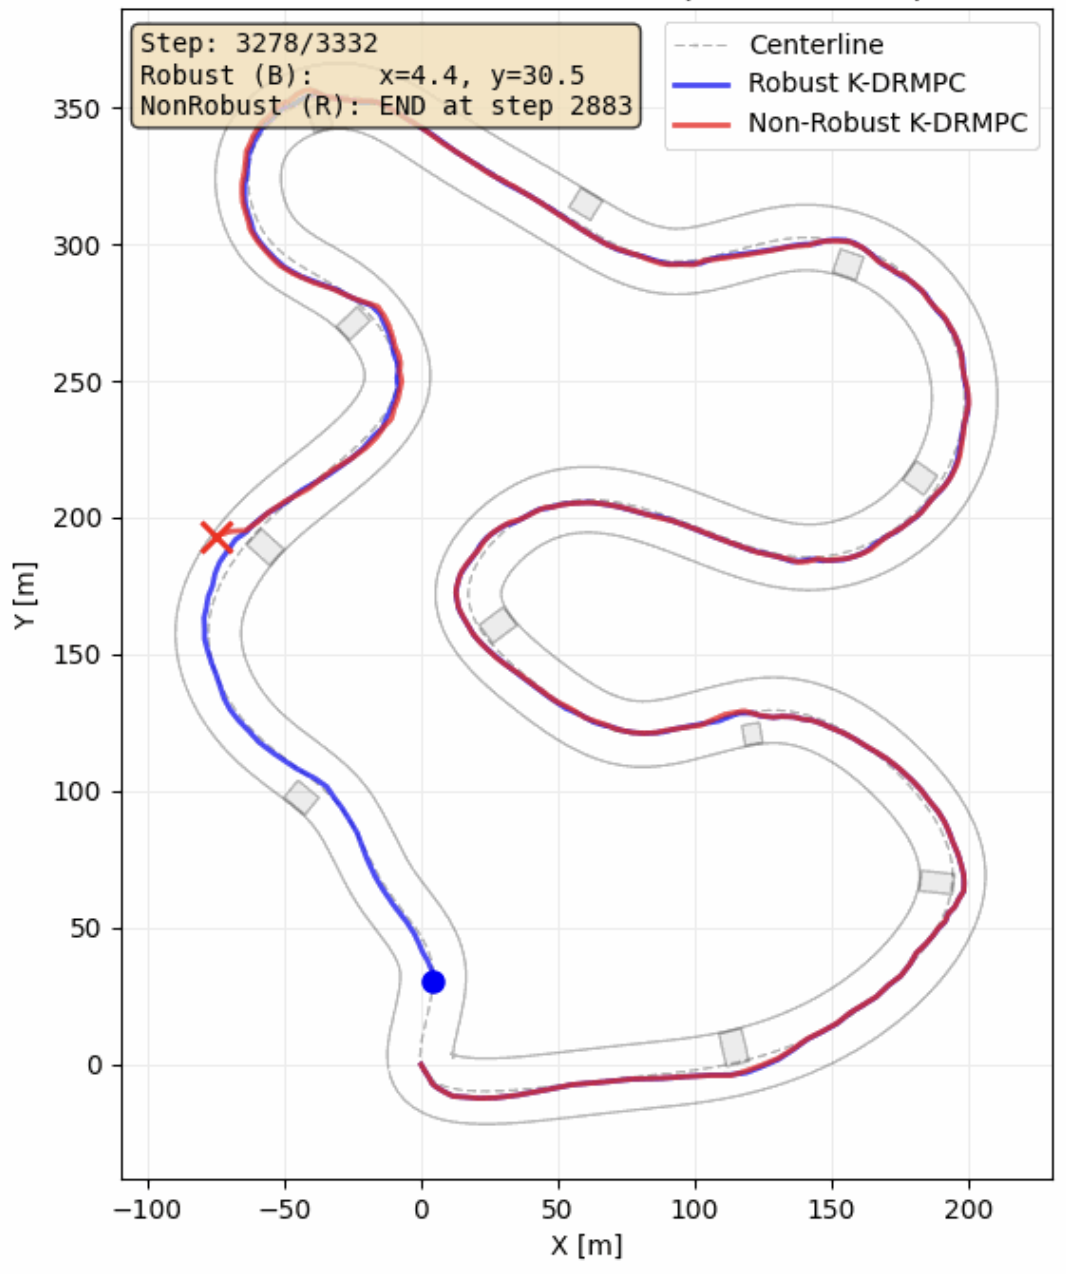
\includegraphics[width=0.5\linewidth]{figures/fig_closed_loop_trajectory_primary.png}
		\caption{Closed-loop trajectory on the primary scenario. The dashed curve is the reference centerline of a preplanned serpentine track, and about 10 gray rectangles denote the fixed static obstacles used throughout the experiments.}
		\label{fig:traj_main}
	\end{figure}

	Table~\ref{tab:main_results} reports the core closed-loop outcomes for K-MPC and K-DRMPC across three disturbance settings (A: nominal, B: moderate shift, C: severe shift), enabling direct comparison of robustness performance under distributional changes.
	For Setting C, note that early termination appears in repeated runs (all K-MPC runs and part of K-DRMPC runs); therefore, trajectory-averaged metrics are computed over truncated horizons and are not strictly comparable to full-horizon runs.
	
	\begin{table*}[htbp]
		\centering
		\caption{Closed-loop performance comparison across Settings A, B, C ($\theta=0.10$, $\epsilon=0.10$).}
		\label{tab:main_results}
		\scriptsize
		\setlength{\tabcolsep}{2.5pt}
		\begin{tabular*}{\textwidth}{@{\extracolsep{\fill}}p{2.8cm}|c c|c c|c c}
			\toprule
			\multirow{2}{*}{\textbf{Metric}} & \multicolumn{2}{c|}{\textbf{Setting A (Nominal)}} & \multicolumn{2}{c|}{\textbf{Setting B (Moderate Shift)}} & \multicolumn{2}{c}{\textbf{Setting C (Severe Shift)}} \\
			\cmidrule{2-7}
			& \textbf{K-MPC} & \textbf{K-DRMPC} & \textbf{K-MPC} & \textbf{K-DRMPC} & \textbf{K-MPC} & \textbf{K-DRMPC} \\
			\midrule
			\multicolumn{7}{l}{\textit{Trajectory Completion}} \\
			Steps & 3378.7 & 3371.0 & 3401.0 & 3387.3 & 1198.3 & 2397.0 \\
			Task time (s) & 337.9 & 337.1 & 340.1 & 338.7 & 119.8 & 239.7 \\
			Crash (Yes/No) & No & No & No & No & Yes (3/3) & Mixed (1/3) \\
			\midrule
			\multicolumn{7}{l}{\textit{Safety-Margin Statistics}} \\
			$m_{\min}$ (m) & -2.793 & -2.681 & -3.426 & -3.355 & -1.016 & -2.319 \\
			$m_{\mathrm{P05}}$ (m) & -0.361 & -0.506 & -0.503 & -0.633 & 0.852 & 0.062 \\
			\midrule
			\multicolumn{7}{l}{\textit{Lateral Error}} \\
			Mean $|e_y|$ (m) & 1.374 & 1.300 & 1.829 & 1.652 & 2.041 & 2.080 \\
			P95 $|e_y|$ (m) & 3.885 & 3.598 & 4.920 & 4.320 & 6.232 & 5.866 \\
			\midrule
			\multicolumn{7}{l}{\textit{Heading Error}} \\
			Mean $|e_\psi|$ (deg) & 3.048 & 2.772 & 3.923 & 3.531 & 5.685 & 4.333 \\
			P95 $|e_\psi|$ (deg) & 9.825 & 9.252 & 11.986 & 11.052 & 25.534 & 13.127 \\
			\midrule
			\multicolumn{7}{l}{\textit{Velocity \& Computational}} \\
			Mean speed (m/s) & 4.313 & 4.311 & 4.313 & 4.307 & 4.942 & 4.502 \\
			Solve mean (ms) & 1373.9 & 1421.1 & 1358.0 & 1394.6 & 1345.7 & 1392.4 \\
			Solve P95 (ms) & 1493.2 & 1553.2 & 1479.6 & 1523.1 & 1507.0 & 1549.2 \\
			\bottomrule
		\end{tabular*}
	\end{table*}
	
	\begin{figure*}[htbp]
		\centering
		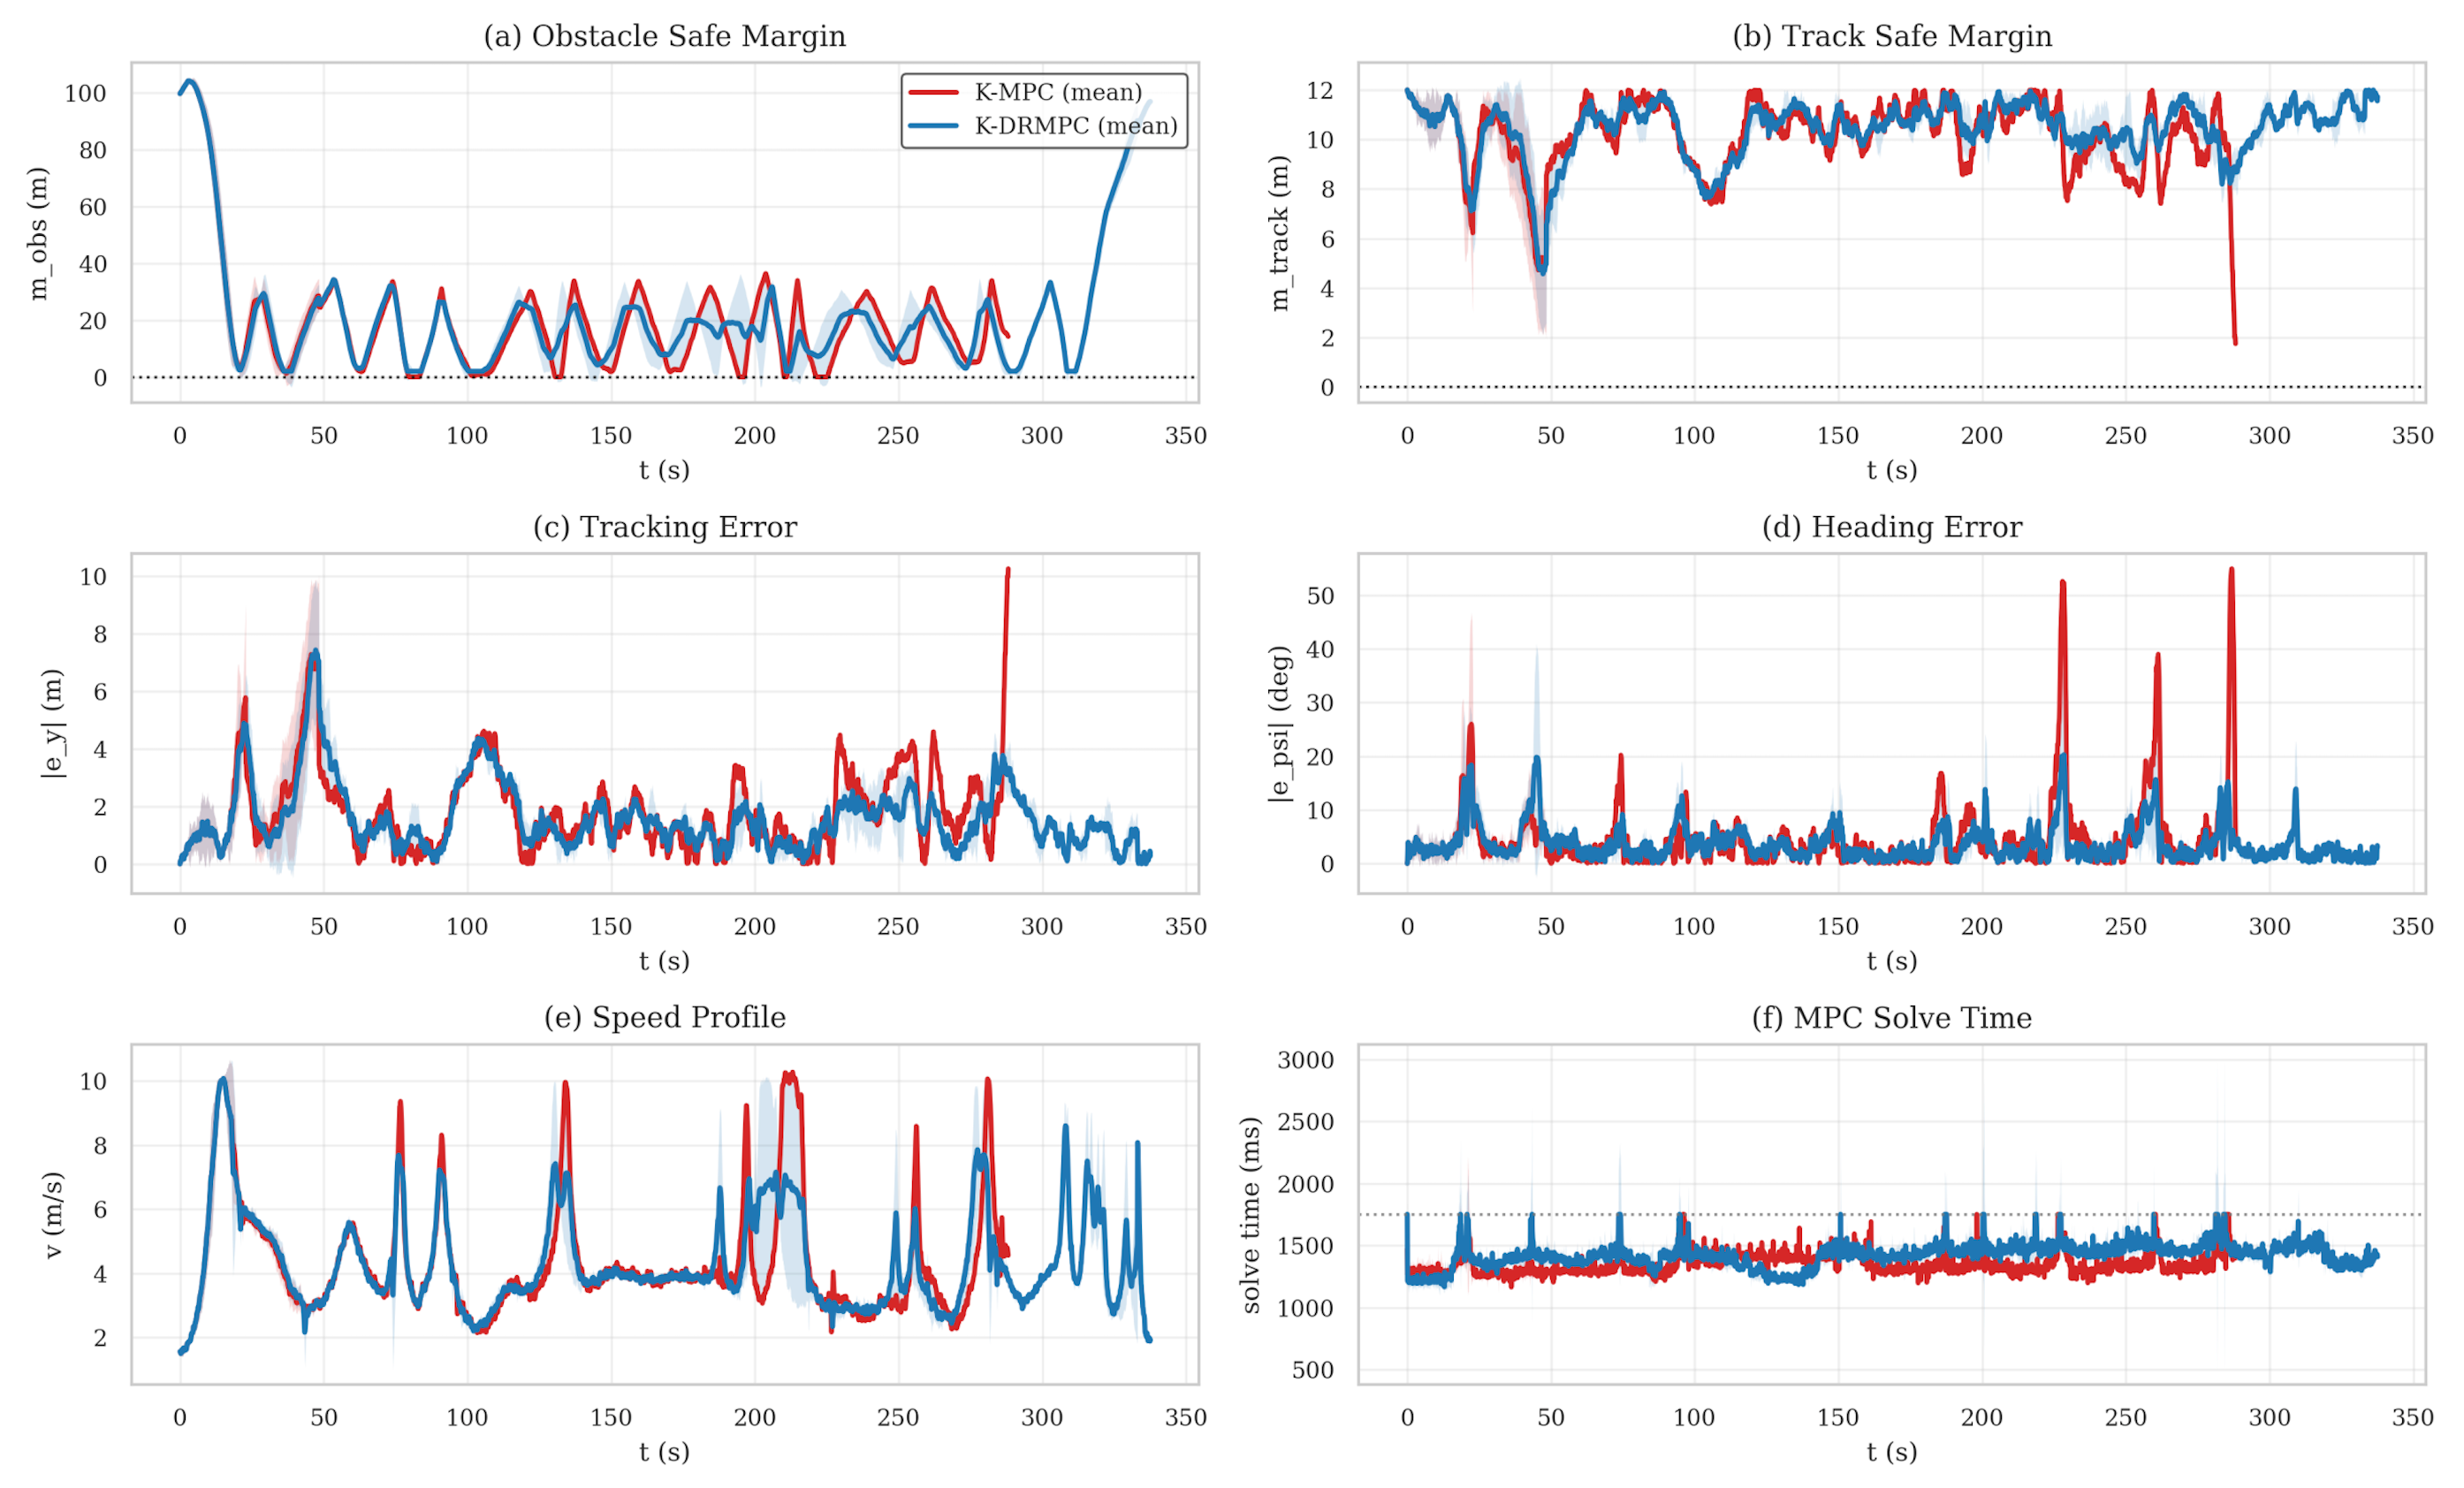
\includegraphics[width=\textwidth]{figures/fig_aggregated_time_series_setting_c.png}
		\caption[Aggregated time-series comparison under Setting C.]{Aggregated time-series comparison between K-MPC and K-DRMPC for Setting C (severe disturbance, $\sigma=1.0$). Curves show run-wise means from the full log batch (three runs per method), with shaded bands indicating dispersion. The safe margin panels (top two) reveal the critical advantage: K-MPC's obstacle and track margins collapse to zero around $t=280$ s, causing mission failure, whereas K-DRMPC maintains positive margins throughout. The remaining four panels report $|e_y|$, $|e_\psi|$, speed profile $v$, and per-step MPC solve time.}
		\label{fig:timeseries_main}
	\end{figure*}
	
	\textit{Parameter sensitivity analysis:}	
To characterize the internal robustness trade-off of K-DRMPC, we sweep the Wasserstein radius $\theta \in \{0.0, 0.5, 1.0, 1.5, 2.0\}$ and the chance constraint risk level $\epsilon \in \{0.01, 0.05, 0.10\}$ under Setting B. Figure~\ref{fig:sensitivity_theta_epsilon} summarizes the resulting sensitivity using the lower-tail safety-margin statistic $m_{\mathrm{P05}}$.

\begin{figure}[t]
	\centering
	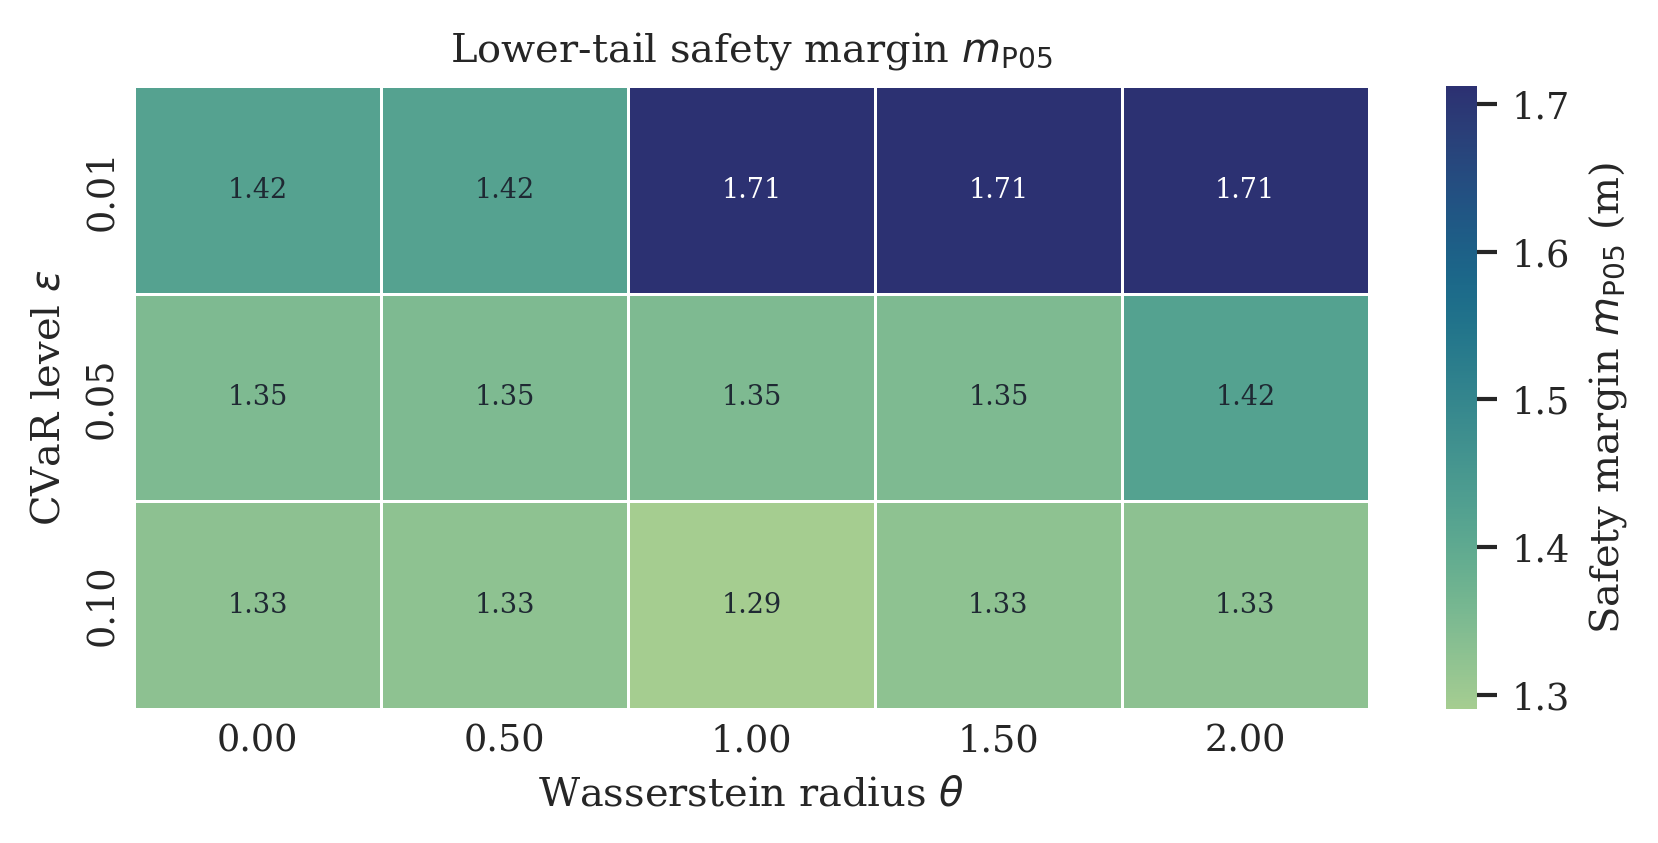
\includegraphics[width=0.8\linewidth]{figures/fig_sensitivity_theta_epsilon.png}
	\caption{Heatmap of the lower-tail safety margin $m_{\mathrm{P05}}$ over the full $(\theta,\epsilon)$ grid under Setting B ($\sigma=0.75$). Each cell reports the realized $m_{\mathrm{P05}}$ for one parameter pair; the color field visualizes how the robustness configuration changes the lower-tail clearance.}
	\label{fig:sensitivity_theta_epsilon}
\end{figure}

During the experiments, we made three main observations. First, all 15 parameter pairs remained feasible, indicating that the controller retains a broad operating region in this moderate-shift regime. Second, $m_{\mathrm{P05}}$ is much more sensitive to $\epsilon$ than to $\theta$: decreasing $\epsilon$ from $0.10$ to $0.01$ consistently increases the lower-tail safety margin, so the chance constraint level is the primary conservatism knob. Third, the effect of $\theta$ is comparatively weak and non-monotone. For example, when $\epsilon=0.10$, the heatmap is nearly flat except for a local dip around $\theta=1.0$; when $\epsilon=0.01$, the margin increases once $\theta$ reaches $1.0$ and then saturates. Overall, $\epsilon$ is the more effective tuning parameter for enlarging realized safety margins, while $\theta$ mainly provides a secondary robustness-shaping effect over the tested range.

In addition, the comparison between robust and non-robust control yields several clear observations. Under the nominal condition (Setting~A), both controllers completed all three runs. K-DRMPC achieved slightly better tracking tails: the mean lateral error dropped from 1.374~m to 1.300~m, and the 95th percentile from 3.885~m to 3.598~m. Heading errors also improved, with the mean and 95th percentile falling from 3.048° and 9.825° to 2.772° and 9.252°, respectively. This came at a computational cost: the mean solve time increased from 1373.9~ms to 1421.1~ms.

Under the moderate shift (Setting~B), both methods still finished all runs, but the robust controller showed larger gains. Its lateral error mean and 95th percentile improved to 1.652~m and 4.320~m, compared to 1.829~m and 4.920~m for K-MPC. The fraction of steps where lateral error stayed within 2~m rose from 66.14\% to 69.91\%. This suggests that the DRO constraints already help under distribution shifts even before any hard failures appear.

The severe shift (Setting~C) produced the clearest difference. K-MPC failed in all three seeds, whereas K-DRMPC completed two of three runs. The robust controller also cut the extreme error tails markedly: the 95th percentile of lateral error went from 6.232~m to 5.866~m, and that of heading error from 25.534° to 13.127°. However, mean error numbers are less comparable here because early termination truncates the trajectories and changes the sample composition. Safety margins such as $m_{\min}$ and $m_{\mathrm{P05}}$ should always be interpreted together with completion status. In Setting~C, the early termination of non-robust runs can artificially inflate quantiles (e.g., giving a positive $m_{\mathrm{P05}}$ despite zero completed runs). Hence, under a severe shift, the completion rate is the primary safety indicator.

From a computational and structural perspective, the Koopman-based formulation strikes a practical balance between model expressiveness and online tractability. Lifting the nonlinear dynamics into a high-dimensional latent space allows MPC to apply linear control theory while preserving global validity. Early-step control decisions and steering-rate constraints have a strong impact on safety and performance. An incorrect steering sign at the beginning can cause an irreversible boundary violation; raising the steering-rate limit could mitigate this. The runtime of K-DRMPC scales with the number of historical disturbance samples (due to the chance constraints, which introduce slack variables $s_{t,i}$) and with the prediction horizon $T$. Across Settings~A–C, the robust overhead in mean solve time ranged from about +36.6~ms to +47.1~ms, and the 95th percentile overhead from +42.2~ms to +60.0~ms.
	
	
	\section{CONCLUSION}
	\label{sec6}
	
	This paper presents a Koopman-based MPC framework for autonomous vehicle obstacle avoidance under disturbance uncertainty. The method combines a finite-dimensional lifted dynamics model, an empirical expected tracking objective, and a Wasserstein ambiguity set for per-step safety constraints. A shifted-hinge loss and Markov's inequality yield conservative sufficient conditions that are affine in the MPC decision variables for fixed margin parameters. The numerical results in this draft were generated before this revised safety condition and must be regenerated before they can be used to evaluate the revised formulation.

The essential difference between the robust and non‑robust controllers is not their nominal accuracy but their reliability as the disturbance magnitude grows. Under nominal conditions, both controllers complete all runs with comparable tracking quality, confirming that robustness does not meaningfully impair normal operation. When the disturbance level increases moderately, K-DRMPC already exhibits a clear advantage in tail errors while still completing every run. Under severe disturbances, the gap becomes decisive: K‑MPC fails in all runs, whereas K‑DRMPC succeeds in two out of three. This outcome indicates that distributional robustness primarily serves as a feasibility‑preserving mechanism, though it incurs a moderate computational overhead. For safety‑critical applications, completion under large disturbances must therefore take precedence over single‑metric averages, and margin quantiles should always be interpreted alongside truncation and crash information.

\enterbackmatter

\supphead{Funding}

This work was supported by the National Natural Science Foundation of China (No. 52432012).

\supphead{Data availability}

The source code and the simulation data necessary to reproduce the findings of this study are publicly available in the GitHub repository https://github.com/xuenanhkust163/Koopman-DRMPC-ObstacleAvoidance.
	
	%% References
	\begin{thebibliography}{99}
		
		\bibitem[Koopman(1931)]{koopman1931}
		B. O. Koopman, ``Hamiltonian systems and transformation in Hilbert space,''
		\textit{Proc. Natl. Acad. Sci. USA}, vol. 17, no. 5, pp. 315--318, 1931.
		
		\bibitem[Williams et al.(2015)]{williams2015}
		M. O. Williams, I. G. Kevrekidis, and C. W. Rowley,
		``A data–driven approximation of the Koopman operator: Extending dynamic mode decomposition,''
		\textit{J. Nonlinear Sci.}, vol. 25, no. 6, pp. 1307--1346, 2015.
		
		\bibitem[Lusch et al.(2018)]{lusch2018}
		B. Lusch, J. N. Kutz, and S. L. Brunton,
		``Deep learning for universal linear embeddings of nonlinear dynamics,''
		\textit{Nat. Commun.}, vol. 9, no. 1, p. 4950, 2018.
		
		\bibitem[Shi and Meng(2022)]{shi2022}
		H. Shi and M. Q.-H. Meng,
		``Deep Koopman operator with control for nonlinear systems,''
		\textit{IEEE Robot. Autom. Lett.}, vol. 7, no. 3, pp. 7700--7707, 2022.
		
		\bibitem[Wu et al.(2023)]{wu2023}
		C. Gu, T. Zhou, and C. Wu,
		``Deep Koopman traffic modeling for freeway ramp metering,''
		\textit{IEEE Trans. Intell. Transp. Syst.}, vol. 24, no. 6, pp. 6001--6013, 2023.
		
		\bibitem[Zheng et al.(2024)]{zheng2024}
		H. Zheng, Y. Li, L. Zheng, and E. Hashemi,
		``Koopman-based hybrid modeling and zonotopic tube robust MPC for motion control of automated vehicles,''
		\textit{IEEE Trans. Intell. Transp. Syst.}, vol. 25, no. 10, pp. 13598--13612, 2024.
		
		\bibitem[Zhang et al.(2022)]{zhang2022}
		X. Zhang, W. Pan, R. Scattolini, S. Yu, and X. Xu,
		``Robust tube-based model predictive control with Koopman operators,''
		\textit{Automatica}, vol. 137, p. 110114, 2022.
		
		\bibitem[Xiao et al.(2022)]{xiao2022}
		X. Xiao, Y. Zhang, and J. Wang,
		``Deep neural networks with Koopman operators for modeling and control of autonomous vehicles,''
		\textit{IEEE Trans. Intell. Veh.}, vol. 7, no. 3, pp. 654--665, 2022.
		
		\bibitem[Esfahani and Kuhn(2018)]{esfahani2018}
		P. M. Esfahani and D. Kuhn,
		``Data-driven distributionally robust optimization using the Wasserstein metric: Performance guarantees and tractable reformulations,''
		\textit{Math. Program.}, vol. 171, no. 1, pp. 115--166, 2018.
		
		\bibitem[Li et al.(2021)]{li2021}
		B. Li, Y. Tan, A.-G. Wu, and G.-R. Duan,
		``A distributionally robust optimization based method for stochastic model predictive control,''
		\textit{IEEE Trans. Autom. Control}, vol. 67, no. 11, pp. 5762--5777, 2021.
		
		\bibitem[Hakobyan and Yang(2023)]{hakobyan2023}
		A. Hakobyan and I. Yang,
		``Wasserstein distributionally robust motion control for collision avoidance using conditional value-at-risk,''
		\textit{IEEE Trans. Robot.}, vol. 39, no. 4, pp. 2690--2707, 2023.
		
		\bibitem[Chen et al.(2024)]{chen2024}
		L. Chen, Y. Liu, and Z. Li,
		``Distributionally robust motion planning for autonomous driving in uncertain environments,''
		\textit{IEEE Trans. Intell. Transp. Syst.}, vol. 25, no. 1, pp. 567--578, 2024.
		
		\bibitem[Mayne et al.(2000)]{mayne2000}
		D. Q. Mayne, J. B. Rawlings, C. V. Rao, and P. O. M. Scokaert,
		``Constrained model predictive control: Stability and optimality,''
		\textit{Automatica}, vol. 36, no. 6, pp. 789--814, 2000.
		
		\bibitem[Rawlings et al.(2017)]{rawlings2017}
		J. B. Rawlings, D. Q. Mayne, and M. M. Diehl,
		\textit{Model Predictive Control: Theory, Computation, and Design}, 2nd ed.
		Santa Barbara, CA, USA: Nob Hill Publishing, 2017.
		
		\bibitem[Zhang et al.(2021)]{zhang2021}
		X. Zhang, X. Xu, and S. Yu,
		``Koopman model predictive control for nonlinear systems,''
		\textit{Automatica}, vol. 132, p. 109800, 2021.
		
		\bibitem[Li et al.(2023)]{li2023}
		B. Li, T. Guan, L. Dai, and G.-R. Duan,
		``Distributionally robust model predictive control with output feedback,''
		\textit{IEEE Trans. Autom. Control}, vol. 68, no. 9, pp. 5443--5458, 2023.
		
		\bibitem[Wang et al.(2024)]{wang2024}
		Y. Wang, X. Zhang, and J. Wang,
		``Data-driven predictive control for autonomous vehicles using Koopman operator,''
		\textit{IEEE Trans. Intell. Transp. Syst.}, vol. 25, no. 2, pp. 1234--1245, 2024.
		
		\bibitem[Liu et al.(2024)]{liu2023}
		J. Liu, X. Zhao, B. Zhu, J. Zhao, and W. Deng,
		``Model predictive control of vehicle dynamics based on the Koopman operator with extended dynamic mode decomposition,''
		\textit{IEEE Access}, vol. 12, pp. 57557--57568, 2024.
		
		\bibitem[Werling et al.(2010)]{werling2010}
		M. Werling, J. Ziegler, S. Kammel, and S. Thrun,
		``Optimal trajectory generation for dynamic street scenarios via convex optimization,''
		in \textit{Proc. IEEE Int. Conf. Robot. Autom. (ICRA)}, Anchorage, AK, USA, May 2010, pp. 5016--5022.
		
		\bibitem[Werling et al.(2010b)]{werling2010b}
		M. Werling, G. Hoffmann, B. Spillmann, and S. Thrun,
		``Online trajectory planning and tracking for autonomous off-road vehicles,''
		in \textit{Proc. IEEE Int. Conf. Robot. Autom. (ICRA)}, Anchorage, AK, USA, May 2010, pp. 5084--5089.
		
		\bibitem[Abtahi et al.(2025)]{abtahi2025}
		M. Abtahi, F. Motallebi Araghi, N. Mojahed, and S. Nazari,
		``Deep bilinear Koopman model for real-time vehicle control in Frenet frame,''
		\textit{IEEE Trans. Intell. Veh.}, under review, 2025.
		[Online]. Available: arXiv:2507.12578.
		
		\bibitem[Chen and Lv(2024)]{chenlv2024}
		H. Chen and C. Lv,
		``Incorporating ESO into deep Koopman operator modelling for control of autonomous vehicles,''
		arXiv preprint arXiv:2405.10157, 2024.
		
		\bibitem[Fang et al.(2026)]{fang2026}
		S. Fang, X. Li, C. Wu, and K. Yu,
		``DRCC-LPVMPC: Robust data-driven control for autonomous driving and obstacle avoidance,''
		arXiv preprint arXiv:2603.14408, 2026.

		\bibitem[Vangasse et al.(2024)]{vangasse2024}
		A. da C. Vangasse, E. J. R. Freitas, G. V. Raffo, and L. C. A. Pimenta,
		``Safe Navigation on Path-Following Tasks: A Study of MPC-based Collision Avoidance Schemes in Distributed Robot Systems,''
		\textit{J. Intell. Robot. Syst.}, vol. 110, no. 4, 2024, doi: 10.1007/s10846-024-02202-3.

		\bibitem[Chen et al.(2026)]{chenjirs2026}
		J. Chen, H. Ebel, and P. Eberhard,
		``Practical Insights on Data-Based Robot Control: A Comparative Analysis of Data-Enabled Predictive Control and Model-Based Predictive Control,''
		\textit{J. Intell. Robot. Syst.}, vol. 112, no. 2, 2026, doi: 10.1007/s10846-026-02386-w.

		\bibitem[Weiss and Behl(2026)]{weiss2026}
		T. Weiss and M. Behl,
		``BARTe: Composite Bezier Curves for Racing Trajectory Estimation,''
		\textit{J. Intell. Robot. Syst.}, vol. 112, no. 2, 2026, doi: 10.1007/s10846-026-02368-y.
		
		\bibitem[Nezami et al.(2024)]{nezami2024}
		M. Nezami, D. S. Karachalios, G. Schildbach, and H. S. Abbas,
		``Obstacle Avoidance of Autonomous Vehicles: An LPVMPC with Scheduling Trust Region,''
		arXiv preprint arXiv:2405.02030, 2024.
		
		\bibitem[Zhu and Borrelli(2024)]{zhu2024}
		E. L. Zhu and F. Borrelli,
		``A sequential quadratic programming approach to the solution of open-loop generalized Nash equilibria for autonomous racing,''
		arXiv preprint arXiv:2404.00186, 2024.
		
		\bibitem[Xue et al.(2024)]{xue2024}
		H. Xue, E. L. Zhu, J. M. Dolan, and F. Borrelli,
		``Learning model predictive control with error dynamics regression for autonomous racing,''
		in \textit{Proc. IEEE Int. Conf. Robot. Autom. (ICRA)}, Yokohama, Japan, May 2024, pp. 4614--4620.
		
		\bibitem[Numerow et al.(2024)]{numerow2024}
		L. Numerow, A. Zanelli, A. Carron, and M. N. Zeilinger,
		``Inherently robust suboptimal MPC for autonomous racing with anytime feasible SQP,''
		arXiv preprint arXiv:2401.02194, 2024.

		\bibitem{Esfahani2018}
		Peyman Mohajerin Esfahani and Daniel Kuhn,
		\emph{Data-driven distributionally robust optimization using the Wasserstein metric: performance guarantees and tractable reformulations},
		Mathematical Programming, vol. 171, no. 1, pp. 115–166, 2018.

		\bibitem{Xie2019}
		Weijun Xie,
		\emph{On distributionally robust chance constrained programs with Wasserstein distance},
		Mathematical Programming, vol. 186, pp. 115–155, 2021.
		(Published online 13 November 2019)
		
	\end{thebibliography}
	
\end{document}
